%%%%%%%%%%%%%%%%%%%%%%%%%%%%%%%%%%%%%%%%%
% Masters/Doctoral Thesis 
% LaTeX Template
% Version 2.5 (27/8/17)
%
% This template was downloaded from:
% http://www.LaTeXTemplates.com
%
% Version 2.x major modifications by:
% Vel (vel@latextemplates.com)
%
% This template is based on a template by:
% Steve Gunn (http://users.ecs.soton.ac.uk/srg/softwaretools/document/templates/)
% Sunil Patel (http://www.sunilpatel.co.uk/thesis-template/)
%
% Template license:
% CC BY-NC-SA 3.0 (http://creativecommons.org/licenses/by-nc-sa/3.0/)
%
%%%%%%%%%%%%%%%%%%%%%%%%%%%%%%%%%%%%%%%%%

%----------------------------------------------------------------------------------------
%	PACKAGES AND OTHER DOCUMENT CONFIGURATIONS
%----------------------------------------------------------------------------------------

\documentclass[
11pt, % The default document font size, options: 10pt, 11pt, 12pt
oneside, % Two side (alternating margins) for binding by default, uncomment to switch to one side
english, % ngerman for German
singlespacing, % Single line spacing, alternatives: onehalfspacing or doublespacing
%draft, % Uncomment to enable draft mode (no pictures, no links, overfull hboxes indicated)
%nolistspacing, % If the document is onehalfspacing or doublespacing, uncomment this to set spacing in lists to single
%liststotoc, % Uncomment to add the list of figures/tables/etc to the table of contents
%toctotoc, % Uncomment to add the main table of contents to the table of contents
%parskip, % Uncomment to add space between paragraphs
%nohyperref, % Uncomment to not load the hyperref package
headsepline, % Uncomment to get a line under the header
%chapterinoneline, % Uncomment to place the chapter title next to the number on one line
%consistentlayout, % Uncomment to change the layout of the declaration, abstract and acknowledgements pages to match the default layout
]{MastersDoctoralThesis} % The class file specifying the document structure

\usepackage[utf8]{inputenc} % Required for inputting international characters
\usepackage[T1]{fontenc} % Output font encoding for international characters
\usepackage{xcolor}
\usepackage{mathpazo} % Use the Palatino font by default
\usepackage{float}
\usepackage[backend=bibtex,style=authoryear,natbib=true]{biblatex} % Use the bibtex backend with the authoryear citation style (which resembles APA)
\usepackage{caption}
\usepackage{subcaption}
\addbibresource{example.bib} % The filename of the bibliography

\usepackage[autostyle=true]{csquotes} % Required to generate language-dependent quotes in the bibliography

%----------------------------------------------------------------------------------------
%	MARGIN SETTINGS
%----------------------------------------------------------------------------------------

\geometry{
	paper=a4paper, % Change to letterpaper for US letter
	inner=2.5cm, % Inner margin
	outer=3.8cm, % Outer margin
	bindingoffset=.5cm, % Binding offset
	top=1.5cm, % Top margin
	bottom=1.5cm, % Bottom margin
	%showframe, % Uncomment to show how the type block is set on the page
}

%----------------------------------------------------------------------------------------
%	THESIS INFORMATION
%----------------------------------------------------------------------------------------

\thesistitle{Sequence Model Evolution:\\ A Time Series Analysis Viewpoint} % Your thesis title, this is used in the title and abstract, print it elsewhere with \ttitle
\supervisor{Dr. Xinyue \textsc{Li}} % Your supervisor's name, this is used in the title page, print it elsewhere with \supname
\examiner{} % Your examiner's name, this is not currently used anywhere in the template, print it elsewhere with \examname
\degree{Master of Science in Data Science} % Your degree name, this is used in the title page and abstract, print it elsewhere with \degreename
\author{Zeyin \textsc{Lin} \\
Yuzhan \textsc{Liu} \\
Ziyi \textsc{Pu}
} % Your name, this is used in the title page and abstract, print it elsewhere with \authorname
\addresses{} % Your address, this is not currently used anywhere in the template, print it elsewhere with \addressname

\subject{SDSC6002 Research Projects for Data Science} % Your subject area, this is not currently used anywhere in the template, print it elsewhere with \subjectname
\keywords{} % Keywords for your thesis, this is not currently used anywhere in the template, print it elsewhere with \keywordnames
\university{\href{https://www.cityu.edu.hk/}{City University of Hong Kong}} % Your university's name and URL, this is used in the title page and abstract, print it elsewhere with \univname
\department{\href{https://www.sdsc.cityu.edu.hk/}{School of Data Science}} % Your department's name and URL, this is used in the title page and abstract, print it elsewhere with \deptname
% \group{\href{http://researchgroup.university.com}{Research Group Name}} % Your research group's name and URL, this is used in the title page, print it elsewhere with \groupname

\AtBeginDocument{
\hypersetup{pdftitle=\ttitle} % Set the PDF's title to your title
\hypersetup{pdfauthor=\authorname} % Set the PDF's author to your name
\hypersetup{pdfkeywords=\keywordnames} % Set the PDF's keywords to your keywords
}

\begin{document}

\frontmatter % Use roman page numbering style (i, ii, iii, iv...) for the pre-content pages

\pagestyle{plain} % Default to the plain heading style until the thesis style is called for the body content

%----------------------------------------------------------------------------------------
%	TITLE PAGE
%----------------------------------------------------------------------------------------

\begin{titlepage}
\begin{center}

\vspace*{.06\textheight}
{\scshape\LARGE \univname\par}\vspace{1.5cm} % University name
\textsc{\Large Research Project Report}\\[0.5cm] % Thesis type

\HRule \\[0.4cm] % Horizontal line
{\huge \bfseries \ttitle\par}\vspace{0.4cm} % Thesis title
\HRule \\[1.5cm] % Horizontal line
 
\begin{minipage}[t]{0.4\textwidth}
\begin{flushleft} \large
\emph{Author:}\\
\authorname % Author name - remove the \href bracket to remove the link
\end{flushleft}
\end{minipage}
\begin{minipage}[t]{0.4\textwidth}
\begin{flushright} \large
\emph{Supervisor:} \\
\href{https://www.cityu.edu.hk/stfprofile/xinyueli.htm}{\supname} % Supervisor name - remove the \href bracket to remove the link  
\end{flushright}
\end{minipage}\\[3cm]
 
\vfill

\large \textit{\degreename}\\[0.3cm] % University requirement text
% \textit{in the}\\[0.4cm]
\deptname\\[2cm] % Research group name and department name
 
\vfill

{\large \today}\\[4cm] % Date
%\includegraphics{Logo} % University/department logo - uncomment to place it
 
\vfill
\end{center}
\end{titlepage}

%----------------------------------------------------------------------------------------
%	DECLARATION PAGE
%----------------------------------------------------------------------------------------

% \begin{declaration}
% \addchaptertocentry{\authorshipname} % Add the declaration to the table of contents
% \noindent I, \authorname, declare that this thesis titled, \enquote{\ttitle} and the work presented in it are my own. I confirm that:

% \begin{itemize} 
% \item This work was done wholly or mainly while in candidature for a research degree at this University.
% \item Where any part of this thesis has previously been submitted for a degree or any other qualification at this University or any other institution, this has been clearly stated.
% \item Where I have consulted the published work of others, this is always clearly attributed.
% \item Where I have quoted from the work of others, the source is always given. With the exception of such quotations, this thesis is entirely my own work.
% \item I have acknowledged all main sources of help.
% \item Where the thesis is based on work done by myself jointly with others, I have made clear exactly what was done by others and what I have contributed myself.\\
% \end{itemize}
 
% \noindent Signed:\\
% \rule[0.5em]{25em}{0.5pt} % This prints a line for the signature
 
% \noindent Date:\\
% \rule[0.5em]{25em}{0.5pt} % This prints a line to write the date
% \end{declaration}

% \cleardoublepage

%----------------------------------------------------------------------------------------
%	QUOTATION PAGE
%----------------------------------------------------------------------------------------

% \vspace*{0.2\textheight}

% \noindent\enquote{\itshape Thanks to my solid academic training, today I can write hundreds of words on virtually any topic without possessing a shred of information, which is how I got a good job in journalism.}\bigbreak

% \hfill Dave Barry

%----------------------------------------------------------------------------------------
%	ABSTRACT PAGE
%----------------------------------------------------------------------------------------

\begin{abstract}
\addchaptertocentry{\abstractname} % Add the abstract to the table of contents
The Thesis Abstract is written here (and usually kept to just this page). The page is kept centered vertically so can expand into the blank space above the title too\ldots
\end{abstract}

%----------------------------------------------------------------------------------------
%	ACKNOWLEDGEMENTS
%----------------------------------------------------------------------------------------

% \begin{acknowledgements}
% \addchaptertocentry{\acknowledgementname} % Add the acknowledgements to the table of contents
% The acknowledgments and the people to thank go here, don't forget to include your project advisor\ldots
% \end{acknowledgements}

%----------------------------------------------------------------------------------------
%	LIST OF CONTENTS/FIGURES/TABLES PAGES
%----------------------------------------------------------------------------------------

\tableofcontents % Prints the main table of contents

% \listoffigures % Prints the list of figures

% \listoftables % Prints the list of tables

% %----------------------------------------------------------------------------------------
% %	ABBREVIATIONS
% %----------------------------------------------------------------------------------------

% \begin{abbreviations}{ll} % Include a list of abbreviations (a table of two columns)

% \textbf{LAH} & \textbf{L}ist \textbf{A}bbreviations \textbf{H}ere\\
% \textbf{WSF} & \textbf{W}hat (it) \textbf{S}tands \textbf{F}or\\

% \end{abbreviations}

% %----------------------------------------------------------------------------------------
% %	PHYSICAL CONSTANTS/OTHER DEFINITIONS
% %----------------------------------------------------------------------------------------

% \begin{constants}{lr@{${}={}$}l} % The list of physical constants is a three column table

% % The \SI{}{} command is provided by the siunitx package, see its documentation for instructions on how to use it

% Speed of Light & $c_{0}$ & \SI{2.99792458e8}{\meter\per\second} (exact)\\
% %Constant Name & $Symbol$ & $Constant Value$ with units\\

% \end{constants}

% %----------------------------------------------------------------------------------------
% %	SYMBOLS
% %----------------------------------------------------------------------------------------

% \begin{symbols}{lll} % Include a list of Symbols (a three column table)

% $a$ & distance & \si{\meter} \\
% $P$ & power & \si{\watt} (\si{\joule\per\second}) \\
% %Symbol & Name & Unit \\

% \addlinespace % Gap to separate the Roman symbols from the Greek

% $\omega$ & angular frequency & \si{\radian} \\

% \end{symbols}

% %----------------------------------------------------------------------------------------
% %	DEDICATION
% %----------------------------------------------------------------------------------------

% \dedicatory{For/Dedicated to/To my\ldots} 

%----------------------------------------------------------------------------------------
%	THESIS CONTENT - CHAPTERS
%----------------------------------------------------------------------------------------

\mainmatter % Begin numeric (1,2,3...) page numbering

\pagestyle{thesis} % Return the page headers back to the "thesis" style

% Include the chapters of the thesis as separate files from the Chapters folder
% Uncomment the lines as you write the chapters

% Chapter 1

\chapter{Introduction to Time Series and Sequential Modeling} % Main chapter title

\label{Chapter1} % For referencing the chapter elsewhere, use \ref{Chapter1} 

%----------------------------------------------------------------------------------------

% Define some commands to keep the formatting separated from the content 
\newcommand{\keyword}[1]{\textbf{#1}}
\newcommand{\tabhead}[1]{\textbf{#1}}
\newcommand{\code}[1]{\texttt{#1}}
\newcommand{\file}[1]{\texttt{\bfseries#1}}
\newcommand{\option}[1]{\texttt{\itshape#1}}

%----------------------------------------------------------------------------------------

\section{What Is A Time Series}

A time series is a sequential set of data points, measured typically over successive times. Most commonly, a time series is a sequence taken at successive equally spaced points in time. So it is a sequence of discrete-time data. In our daily life, observing data at various points in time is a common activity. Time series data can be found in many fields such as agriculture, economics, meteorology and military. For example, the ancient Egyptians recorded the fluctuations of the Nile River day by day, it is a time series. The sequence of daily closing prices of the Google Inc. stock is a time series. The heart rate monitoring records is a time series.

Once a time series is collected or measured, the primary goal is to analyze the time series and forecast the future values of the time series. Time series analysis comprises methods for analyzing time series data in order to extract meaningful statistics and other characteristics of the data. In the development process of time series analysis methods, the application of economics, finance, engineering and other fields has always played an important role in promoting, and every step of the development of time series analysis is inseparable from the application. 

Time series forecasting is the use of a model to predict future values based on previously observed values. One of biggest differences between time series data and other types of data is that time series data have a natural temporal ordering, the data value at the current moment is related to the data value at the previous moment. This feature indicates that the past data has hinted the law of current or future data development.

% defination
\subsection{Categories}
Methods of time series analysis can be divided into univariate and multivariate, linear and non-linear, discrete and continuous.
\begin{itemize}
    \item Univariate vs. multivariate. A time series containing records of a single variable is termed as univariate, but if records of more than one variable are considered then it is termed as multivariate, multivariate time series model is an extension of the univariate case.
    \item Linear vs. non-linear. A time series model is said to be linear or non-linear depending on whether the current value of the series is a linear or non-linear function of past observations.
    \item Discrete vs. continuous. In a continuous time series observations are measured at every instance of time, whereas a discrete time series contains
    observations measured at discrete points in time.
\end{itemize}

\subsection{Components of a Time Series}
An observed time series can be decomposed into four components: the trend (long term direction), the seasonal variations (systematic, calendar related movements), the cyclical variation (periodical but not seasonal), and the irregular variation (unsystematic, short term fluctuations). Each expressing a particular aspect of the movement of the values of the time series. 

\subsubsection{Trend}
The trend shows the general tendency of the data to increase or decrease during a long period of time. A trend is a smooth, general, long-term, average tendency. It is not always necessary that the increase or decrease is in the same direction throughout the given period of time.

It is observable that the tendencies may increase, decrease or are stable in different sections of time. But the overall trend must be upward, downward or stable. The population, agricultural production, items manufactured, number of births and deaths, number of industry or any factory, number of schools or colleges are some of its example showing some kind of tendencies of movement.
\subsubsection{Seasonal variation}
These are the rhythmic forces which operate in a regular and periodic manner over a span of less than a year. They have the same or almost the same pattern during a period of 12 months. This variation will be present in a time series if the data are recorded hourly, daily, weekly, quarterly, or monthly.
These variations come into play either because of the natural forces or man-made conventions. The various seasons or climatic conditions play an important role in seasonal variations. Such as production of crops depends on seasons, the sale of umbrella and raincoats in the rainy season, and the sale of electric fans and A.C. shoots up in summer seasons.
\subsubsection{Cyclical variation}
The variations in a time series which operate themselves over a span of more than one year are the cyclic variations. This oscillatory movement has a period of oscillation of more than a year. One complete period is a cycle.
\subsubsection{Irregular variation}
There is another factor which causes the variation in the variable under study. They are not regular variations and are purely random or irregular. These fluctuations are unforeseen, uncontrollable, unpredictable, and are erratic. 

\section{How to identify time series anomaly period}

Time series anomaly detection can be transformed into a task where the goal is to model the time series; and given this model, it finds periods where the predicted values are significantly different from the others. Traditionally, researchers use ARMA, ARIMA, GARCH, and other statistics-based methods to do modeling tasks. And following are some common approaches to use for anomaly detection:
\subsubsection{Model-based method}
Determine whether the sample point is an abnormal sample by judging whether the difference between the sample value and the expected value exceeds the critical value. This method can be divided into estimation models and prediction models by different ways to get expectations. For example, a common method to define outliers is the “3 times the standard deviation”rule, often referred to as the three-sigma rule of thumb. If this absolute value is more than 3 times the standard deviation of our values, then we can consider the value as an outlier or anomaly. Except this, a box plot or boxplot is a method for graphically depicting groups of numerical data through their quartiles, which can be used to find anomaly points. Grubbs' s test, also known as the maximum normalized residual test or extreme studentized deviate test, is a test used to detect outliers in a univariate data set assumed to come from a normally distributed population.

\subsubsection{Density-based method}
The density estimation of the object can be calculated relatively directly, especially when there is a proximity measure between the objects, the object in the low-density area is relatively far away from the neighbors, which may be regarded as abnormal. A more sophisticated method takes into account the fact that the data set may have regions of different density, and classifies a point as an outlier only when its local density is significantly lower than most of its neighbors.

\subsubsection{Cluster-based method}
One way to use clustering to detect outliers is to discard small clusters that are far away from other clusters. This method can be used with any clustering method, but requires the minimum cluster size and the national value of the distance between small clusters and other clusters. Generally, the process can be simplified to discard all clusters smaller than a certain minimum size. This scheme is highly sensitive to the choice of the number of clusters.

\subsubsection{Partition-based method}
The partition-based method is used for anomaly detection, which is often very interpretable and easy to operate at the same time. The simplest division method is threshold detection, which sets thresholds through human experience and judges data abnormalities.

Specifically, in order to avoid false alarms caused by single-point jitter, it is necessary to determine the average value of the accumulated window for threshold judgment, and the specific accumulation is to operate through the window. There are many optional choices for the statistical characteristics of the window, such as moving average, cumulative moving average, weighted moving average,exponential weighted moving average, stddev from average etc. 

\section{Statistical Methods and Comparassion}
The foundation of time series analysis is stationarity. Stationarity can be defined in precise mathematical terms, but for our purpose we mean a flat looking series, without trend, constant variance over time, a constant autocorrelation structure over time and no periodic fluctuations (seasonality).


A time series ${r_t}$ is said to be strictly stationary if the joint distribution of $(r_{t_1}, . . . . . ., r_{t_k})$ is identical to that of $(r_{t_1 + t} , . . . . . ., r_{t_{k}+t})$ for all t, where k is an arbitrary positive integer and $(t_1, . . . . . . , t_k)$ is a collection of k positive integers. This is a very strong condition that is hard to verify empirically. However a time series ${r_t}$ is weakly stationary if both the mean of $r_t$ and the covariance between $r_t$ and $r_{t-l}$ are time invariant, where $l$ is an arbitrary integer. More specifically, ${r_t}$ is weakly stationary if

(a) $E(r_t) = \mu$, which is a constant, and

(b) $Cov( r_t ,  r_{t-l} ) = \gamma_{l} $, which only depends on $l$.

A time series $r_t$ is called a white noise if $\{r_t\}$ is a sequence of independent and identically distributed random variables with finite mean and variance. Here “noise” means there’s no pattern, just random variation. The “white” is because all freqencies are equally represented. This will become clear when we do frequency domain analysis of time series.

If $r_t$ is normally distributed with mean zero and variance $\sigma^2$, the series is called a $\mbox{Gaussian white noise}$.

\subsection{AR and MA}
Two of the most common models in time series are the Autoregressive (AR) models and the Moving Average (MA) models.
\subsubsection{AR}
The basic idea of AR is that we will model the response at time $x_t$ t as a linear function of its $p$ previous values and some independent random noise. We explicitly define an autoregressive model of order $p$, abbreviated as $AR (p)$ as:
$$ (x_t - \mu_x) = \phi_1 (x_{t-1} - \mu_X) + \phi_2 (x_{t-2} - \mu_X) + \cdots + \phi_p (x_{t-p} - \mu_X) + w_t$$
where $\phi_p \neq 0$, $x_t$ is stationary with mean $E[x_t] = \mu_x$, and $w_t \overset{\text{i.i.d}}{\sim} N(0, \sigma_w^2)$

The autoregressive operator notation:
$$ \phi(B) = 1 - \phi_1 B -  \phi_2 B^2 - \cdots  -\phi_p B^p,$$
where $B^p x_t = x_{t-p}$ is the backshift operator. We can rewrite the AR model as $ \phi (B)(x_t - \mu_x) = w_t $.

\subsubsection{MA}
Instead of assuming that elements of a time series $x_t$ are linear function of previous elements of the time series $(x_1, . . . , x_{t−1})$ and independent, identically distributed noise $w_t$, we might assume that elements of a time series $x_t$ are a linear function of all of the current and previous noise variates, $w_1, . . . , w_{t−1}$. The latter gives us the moving average model of order $q$, abbreviated as $MA (q)$. The $MA (q)$ model is explicitly defined as:
$$  x_t - \mu_x =  w_t + \theta_1 w_{t-1} + \theta_2 w_{t-2} + \cdots + \theta_q w_{t-q},$$
where $\theta_q \neq 0$, $E[x_t] = \mu_x$, and $w_t \overset{\text{i.i.d}}{\sim} N(0, \sigma_w^2)$. The moving average operator notation: 
$$ \theta (B) = 1 + \theta_1 B + \theta_2 B^2 + \cdots + \theta_p B^p $$We can rewrite the MA model as $ x_t - \mu_x = \theta(B)w_t$.

\subsection{ARMA and ARIMA}
\subsubsection{ARMA}
The autoregressive moving average (ARMA) model combines the AR and MA models. We define an $ARMA(p, q)$ model as:
$$ (x_t - \mu_x) = \phi_1 (x_{t-1} - \mu_X)  + \cdots + \phi_p (x_{t-p} - \mu_X) +  \theta_1 w_{t-1}  + \cdots + \theta_q w_{t-q} + w_t$$
where $w_t \overset{\text{i.i.d}}{\sim} N(0, \sigma_w^2)$, $x_t$ is stationary, $p$ as the autoregressive
order and $q$ as the moving average order. 

\subsubsection{ARIMA}
ARIMA is an acronym that stands for Auto-Regressive Integrated Moving Average. Specifically, $AR$ means autoregression, $MA$ means moving Average. Here $I$ means integrated, the use of differencing of raw observations in
order to make the time series stationary. Usually, a process $x_t$ is said to be $ARIMA(p, d, q)$ if:
$$ \nabla^d X_t  = (1-B)^d X_t$$
is $ARMA(p,q)$. In general, $ARIMA(p, d, q)$ model can be written as:
$$ \phi (B)(1-B)^d x_t = \theta(B) w_t $$

\subsection{GARCH}
The autoregressive conditional heteroscedasticity (ARCH) model is a statistical model for time series data that describes the variance of the current error term or innovation as a function of the actual sizes of the previous time periods' error terms. The ARCH model is appropriate when the error variance in a time series follows an autoregressive (AR) model; if an autoregressive moving average (ARMA) model is assumed for the error variance, the model is a generalized autoregressive conditional heteroskedasticity (GARCH) model.

Let $Z_t$ be $N(0,1)$. The process $x_t$ is a GARCH(p,q) process if it is stationary and if it satisfies, for all $t$ and some strictly positive-valued process $\sigma_t$, the equations:
$$ x_t  = \sigma_t Z_t$$
$$ \sigma_t^2 = \alpha_0 + \sum_{i = 1}^{q} \alpha_i X_{t-i}^2 + \sum_{j = 1}^{p} \phi_j \sigma_{t-j}^2 $$
where $\alpha_0 > 0$ and $\alpha_i >= 0$, i = $1,\cdots,q$, j = $1,\cdots,p$.
%----------------------------------------------------------------------------------------

\section{Architecture of This Report}
The framework of this report list as follows, and shows in \ref{fig:framework}.

\begin{itemize}
\item Chapter 1: Introduction to sequential modeling and time series anomaly detection
\item Chapter 2: Deep Learning theory and Related Derivative
\item Chapter 3: Experiment 1: TCN in various sequence datasets
\item Chapter 4: Experiment 2: Time series anomaly detection in grid load issue
\item Chapter 5: Conclusion and future directions
\end{itemize}

\begin{figure}[H]
    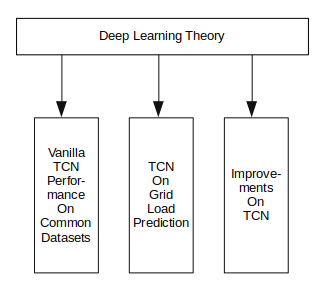
\includegraphics[width=\textwidth]{../Figures/total.png}
    \caption{Total Framework of This Report}
    \label{fig:framework}
\end{figure}

% Chapter 2

\chapter{Deep Learning theory and Related Derivated} % Main chapter title

\label{Chapter2} % For referencing the chapter elsewhere, use \ref{Chapter1} 

\setlength{\parindent}{0pt}
%----------------------------------------------------------------------------------------

\section{Recurrent Neural networks}

Artificial neural networks usually only fetch and process one input individually, and the previous input has nothing to do with the next input. However, some tasks need to handle sequence information better, which means the previous input is related to the subsequent input. In this kind of problem, former researchers Graves and Alex (2009) designed the recurrent neural network (RNN), which is a class of artificial neural networks where connections between nodes form a directed graph along a temporal sequence. This allows it to exhibit temporal dynamic behavior. Derived from feedforward neural networks, RNNs can use their internal state (memory) to process variable-length sequences of inputs.

Sepp Hochreiter and Jürgen Schmidhuber (1997) post the practical method under the concept of RNN, that is, Long short-term memory (LSTM) architecture, with both feedforward neural networks and feedback connections.  This makes them applicable to tasks such as unsegmented, connected handwriting recognition, or speech recognition.

\section{Convolutional Neural Networks and TCN}

Convolutional Neural Networks (CNNs) were originally used on two-dimensional and three-dimensional images, but they are also suitable for one-dimensional data such as univariate time series. Shaojie Bai, J. Zico Kolter, and Vladlen Koltun (2018) designed the architecture temporal convolutional network (TCN) and ran it into image, sound, and text level tasks. This work inspired that convolutional networks could reach the same even better results as other sequence models. Alberto (2019) experimented with TCN and other sequence models in smart grids situations, also found that convolutional networks are significantly useful in time series tasks. However, Seq2Seq methods still hold the best performance place.

\subsection{The origin of TCN}
The Temporal Convolutional Networks (TCNs) was first proposed by the work of Lea et al. (2016) for video-based action segmentation. The two steps of this conventional process include: firstly, computing of low-level features using (usually) CNN that encode spatial-temporal information and secondly, input these low-level features into a classifier that captures high-level temporal information using (usually) RNN. The main disadvantage of such an approach is that it requires two separate models. TCN provides a unified approach to capture all two levels of information hierarchically.

\subsubsection{Encoder-Decoder TCN} The encoder-decoder framework is presented in below, where further information regarding the architecture can be found in the first two references (at the end of the post). The most critical issues are provided as follows: TCN can take a series of any length and output it as the same length. A causal convolutional is used where a 1D fully convolutional network architecture is used. A key characteristic is that the output at time $t$ is only convolved with the elements that occurred before $t$. 
\begin{figure}[H]
    \includegraphics[width=0.9\textwidth]{../Figures/ch3_1.png}
    \caption{Encoder-Decoder TCN}
\end{figure}
The encoder consists of $L$ layers denotes by $E^l \in R^{F_l\times T_l}$ where $F_l$ is the number of convolutional filters in a the $l-th$ layer and $T_l$ is the number of corresponding time steps. Each layer consists of temporal convolutions, a non-linear activation function, and max pooling across time. We define the collection of filters in each layer as $W=W^{(i)F_l}_{i=1}$ for $W^{(i)} \in R ^{d \times F_{l-1}}$ with a corresponding bias vector $b \in R^{F_l}$. Given the signal from the previous layer,$E^{(l-1)}$, we compute $E^{(l)}$activations  with $$E^{(l)} = max pooling(f(W \times E^{(l-1)} + b ))$$, where $f(\cdot)$is the activation function and $\star$ is the (“same”) convolution operator. After each activation function we max pool with width 2 across time so $T_l = \frac{1}{2}T_{l-1}$. Pooling enables us to efficiently compute activations over long temporal windows.

The decoder is similar to the encoder, except that upsampling is used instead of pooling and the order of the operations is now upsample, convolve, and apply the activation function. Upsampling is performed by simply repeating each entry twice. The convolutional filters in the decoder distribute the activations from the condensed layers in the middle to the action predictions at the top. Experimentally, these convolutions provide a large improvement in performance and appear to capture pairwise transitions between actions. Each decoder layer is denoted by $D^{(l)} \in R^{F_l \times T_l}$ for $l \in L,\cdots,1$. Note that these are indexed in reverse order compared to the encoder, so the filter count in the first encoder layer is the same as in the last decoder layer. The probability that frame  corresponds each of the C action classes is given by vector $\hat{Y_t} \in \left[0,1\right]^C$ using weight matrix $U \in R^{C \times F_1}$ and bias $c \in R^C$, such that $$\hat{Y_t} = softmax(UD_t^{(1)}+C)$$
We explored other mechanisms, such as skip connections between layers, different patterns of convolutions, and other normalization schemes, however, the proposed model outperformed these alternatives and is arguably simpler.

\subsubsection{Dilated TCN}
As shown in \ref{fig:dtcn}, we define a series of blocks, each of which contains a sequence of $L$ convolutional layers. The activations in the $l-th$ layer and $j-th$ block are given by $S^{(j,l)} \in R^{(F_w \times T)}$ . The input into each block $S^{(j,1)}$ is the output from the previous block $S^{(j-1,L)}$, except for the first block which is defined as the input data. Each layer has the same number of filters $F_w$, which enables us to combine activations from different layers using skip connections later. Each layer consists a set of dilated convolutions with rate parameter $s$, a non-linear activation $f(\cdot)$, and a residual connection than combines the layer’s input and the convolution signal. Convolutions are only applied over two-time steps, $t$ and $t-s$, so we write out the full equations below. 

The filters are parameterized by $W = \left\{W^{(1)},W^{(2)}\right\}$ with $W^{(i)} \in R^{F_w \times F_w}$ and bias vector $b \in R{F_w}$. Let $\hat{S_t}^{(j,l)}$ be the result of the dilated convolution at time $t$ and $S_t^{j,l}$ be the result after adding the residual connection such that $$\hat{S_t}^{(j,l)} = f(W^{(1)}S_{t-s}^{(j,l-1})+W^{(2)}S_{t}^{(j,l-1})+b)$$
$$ S_t^{\left(j,l\right)}=S_t^{\left(j,l-1\right)}+V{\hat{S}}_t^{\left(j,l\right)}+e $$

Let $V \in R^{F_w \times F_w}$ and $e \in R^{F_w}$ be a set of weights and biases for the residual. Note that parameters $\left\{W,b,V,e\right\}$ are separate for each layer.
The dilation rate increases for consecutive layers within a block such that $s_l = 2$. This enables us to increase the receptive field by a substantial amount without drastically increasing the number of parameters.The output of each block is summed using a set of skip connections with $Z^{(0)} \in R^{(F_w \times T)}$ such that $$Z^{(0)} = ReLU(\sum_{j=1}^B S_t^{(j,l)})$$

There is a set of latent states $Z_t^{(1)} = ReLU(V_rZ_t^{(0)} + e_r)$ for weight matrix $V_r \in R^{F_w \times F_w}$ and bias $e_r$. The predictions for each time $t$ are given by $$\hat{Y_t} = softmax(UZ_t^{(1)}+C)$$ for weight matrix $U \in R^{C \times F_w}$ and bias $c \in R^C$.

\begin{figure}[H]
    \includegraphics[width=0.9\textwidth]{../Figures/ch3_2.png}
    \caption{Dilated TCN}
    \label{fig:dtcn}
\end{figure}

\subsection{Further development and description of TCN}
S. Bai et al. (2018) suggest that convolutional networks should be taken into consideration as one of the primary candidates when modeling sequential data. They were able to show that convolutional networks can achieve better performance than RNNs in many tasks while avoiding common drawbacks of recurrent models, such as the exploding/vanishing gradient problem or lacking memory retention. Furthermore, using a convolutional network instead of a recurrent one can lead to performance improvements as it allows for parallel computation of outputs. They suggest a few additions to the basic TCN architecture for improved performance which will be discussed in this section, namely residual connections, regularization and activation functions.

\subsubsection{Residual Blocks}
The biggest modification we make to the previously introduced basic model is to change the fundamental building block of the model from a simple 1D causal convolutional layer to a residual block which consists of 2 layers with the same dilation factor and a residual connection.

A residual block contains a branch leading out to a series of transformations F, whose outputs are added to the input x of the block: $$o=Activation(x+F(x))$$

Let’s consider a layer with a dilation factor $d$ of 2 and kernel size $k$ of 3 from the basic model to see how this translates into a residual block of the improved model.
\begin{figure}[H]
    \includegraphics[width=\textwidth]{../Figures/ch3_3.png}
    \caption{Residual Blocks}
\end{figure}

The output of the two convolutional layers will be added to the input of the residual block to produce the input for the next block. For all inner blocks of the network, i.e. all but the first and the last one, the input and output channel width is the same, namely num\_filters. Since the first convolutional layer of the first residual block and the second convolutional layer of the last residual block may have different input and output channel widths, the width of the residual tensor might have to be adjusted, which is done using a $1\times1$ convolution.

This change affects the calculus for the minimum number of required layers for full coverage. Now we have to think about how many residual blocks are necessary to achieve a full receptive field coverage. Adding a residual block to a TCN adds twice as much receptive field width than when adding a basic causal layer, since it includes 2 such layers. So the total size of the receptive field r of a TCN with dilation base b, kernel size k with $k \geq b $and number of residual blocks n can be computed as $$r = 1 + \sum_{i=0}^{n-1}2(k-1)b^i=1+2(k-1)\times \frac{b^n-1}{b-1}$$, which leads to a minimum number of residual blocks  for full history coverage of input\_length $l$ of $$n=\left[log_b(\frac{(l-1)(b-1)}{2(k-1)}+1)\right]$$

\subsubsection{Activation, Normalization, Regularization}
To make our TCN more than just an overly complex linear regression model, activation functions need to be added on top of the convolutional layers to introduce non-linearities. $ReLU$ activations are added to the residual blocks after both convolutional layers.

To normalize the input of hidden layers (which counteracts the exploding gradient problem among other things), weight normalization is applied to every convolutional layer.

In order to prevent overfitting, regularization is introduced via dropout after every convolutional layer in every residual block. The following figure shows the final residual block.
\begin{figure}[H]
    \includegraphics[width=\textwidth]{../Figures/ch3_4.png}
    \caption{Final Residual Blocks}
\end{figure}
The asterisk in the second $ReLU$ unit indicates that it is present in every layer but the last one, since we want our final output to be able to take on negative values as well (this differs from the architecture outlined in the paper).

The following picture shows our final TCN model with $l$ equal to input\_length, $k$ equal to kernel\_size, $b$ equal to dilation\_base, $k\geq b$ and with a minimum number of residual blocks for full history coverage, where $n$ can be computed from the other values as explained above.
\begin{figure}[H]
    \includegraphics[width=\textwidth]{../Figures/ch3_5.png}
    \caption{final TCN model}
\end{figure}


\subsection{Applications of TCN}

\subsubsection{Weather prediction}
The buzz around TCN arrives even to Nature journal, with the recent publication of the work by Yan et al. (2020) on TCN for weather prediction tasks. In their work, a comparative experiment was conducted with TCN and LSTM. One of their results was that, among other approaches, the TCN performs well in prediction tasks with time-series data.
In the paper, the author introduces a mode called ensemble empirical mode decomposition (EEMD). EEMD not only can decompose high-frequency time series into some adaptive orthogonal components, called intrinsic mode functions (IMFs), but also has the advantages of noise-assistance and overcoming the drawbacks of mode mixing in conventional empirical mode decomposition (EMD). EEMD can be used to decompose the high-frequency time-series Niño 3.4 index and SOI data into multiple adaptive orthogonal components to improve the prediction accuracy of the model. Therefore, this paper proposes the EEMD-TCN hybrid approach, which is used to decompose the highly variable ENSO indexes (Niño 3.4 index and SOI) into relatively flat subcomponents, and then uses the TCN model to predict each subcomponent in advance, finally combining the sub-prediction results to obtain the final ENSO prediction results.
\begin{figure}[H]
    \includegraphics[width=\textwidth]{../Figures/ch3_6_weather.png}
    \caption{Different model performance in Weather data}
\end{figure}

\subsubsection{Traffic prediction}
Ride-sharing and online navigation services can improve traffic prediction and change the way of life on the road. Fewer traffic jams, less pollution, safe and fast driving are just a few examples of essential issues that can be achieved by better traffic predictions. As this is a real-time data-driven problem, it is necessary to utilize the accumulated data of upcoming traffic. For this reason, Dai et al. (2020) recently presented a Hybrid Spatio-Temporal Graph Convolutional Network (H-STGCN). The general idea is to take the advantages of the piecewise-liner-flow-density relationship and convert the upcoming traffic volume in its equivalent in travel time. One of the most interesting approaches they used in this work is the graph convolution to capture the spatial dependency. The compound adjacency matrix captures the innate characteristics of traffic approximation. In the following architecture, four modules are presented to describe the entire prediction process.\\
In this paper, they describe the overall architecture of H-STGCN, as illustrated in figure below. The model input consists of two feature tensors, the ideal-future-volume tensor $V$ and travel-time tensor $T$. Specifically, both $V$  and $T$ have three dimensions: the spatial dimension, temporal dimension, and channel dimension, which corresponds respectively to the road segments, previous time slots utilized, and features.

\begin{figure}[H]
    \includegraphics[width=\textwidth]{../Figures/ch_3_7_traffic.png}
    \caption{H-STGCN model}
\end{figure}
 \textbf{Historical Average (HA).}  Let $L$ denote the number of time slots in a week. Then the historical average of variable $\omega_{i,t}$ (ideal future: volume or travel time) is given by
$$\omega_{i,t}^{\left(h\right)}={\frac{1}{W}}_{r\equiv t}\sum_{\left(mod\ L\right),r\neq t,r\in\left[0,S_{train}\right)}\omega_{i,t}$$
Where W is the number of weeks in the training set. \\
\textbf{Ideal Future Volume.} As an approximation of the unavailable actual future traffic volume, the ideal future volume $\nu_{i,t_0,f}$can be acquired from an online navigation engine.\\
In H-STGCN, ideal future volume within the prediction window and the corresponding historical average are both taken as input:
$$V_{i,t}=\left[v_{i,t,0},v_{i,t,1},\ldots,v_{i,t,F},v_{i,t,0}^{\left(h\right)},v_{i,t+1,0}^{\left(h\right)},\ldots,v_{i,t+F,0}^{\left(h\right)}\right]$$
where i is the segment index, $\nu_{i,t_0,f}\left(f\geq0\right) $is the counterpart of $\nu_{i,t_0+f}$. \\

\textbf{Travel Time.} Travel time $\tau_{i,t}$ is calculated using the map-matched GPS data from Amap. In H-STGCN, travel time and its historical average within the prediction window are also both taken as input:
$$T_{i,t}=\left[\tau_{i,t},\tau_{i,t}^{\left(h\right)},\tau_{i,t+1}^{\left(h\right)},\ldots,\tau_{i,t+F}^{\left(h\right)}\right]$$
where $i$ is the segment index. \\
 \textbf{Optimization.} For the multistep traffic forecasting task in this paper, they use the $L1 $ loss function:
$$\mathcal{L}=\frac{1}{n\times S_{train}\times F}\sum_{i\in\left[0,n\right),t\in\left[0,S_{train}\right),f\in\left(0,F\ \right]}\left|{\hat{\tau}}_{i,t+f}-\tau_{i,t+f}\right|$$
where ${\hat{\tau}}_{i,t+f}$is the model output and $\tau_{i,t+f}$ is the ground truth.
\subsubsection{Sound event localization and detection}
The field of sound event localization and detection (SELD) continues to grow. Understanding the environment plays a critical role in autonomous navigation. Guirguis et al. (2020) recently proposed a novel architecture for sound events SELD-TCN. They claim that their framework outperforms the state-of-the-art in the field, with faster training time. In their SELDnet (architecture below), a multichannel audio recording, sampled at 44.1 kHz, extracts, by applying a short-time Fourier transformation, the phase and magnitude of the spectrum, and stacks it as separate input features. Then, convolutional blocks and recurrent blocks (bi-directional GRUs) are connected, followed by a fully-connected block. The output of the SELDnet is the SOUND Event Detection (SED) and Direction Of Arrival (DOA).
\begin{figure}[H]
    \includegraphics[width=\textwidth]{../Figures/ch_3_8_sound_1.png}
    \caption{SED and DOA}
\end{figure}
 In order to outperform it, they present the SELD-TCN:
\begin{figure}[H]
    \includegraphics[width=\textwidth]{../Figures/ch_3_9_sound_2.png}
    \caption{SELD-TCN model}
\end{figure}
The aforementioned SELDnet architecture is used while replacing the recurrent block by a TCN, where they adopt the WaveNet architecture. Fig. b shows an overview of the proposed TCN block architecture. Then, to mimic the bidirectional RNNs’ use of future
knowledge, they modify all convolutions within the TCN block to be non-causal. In this implementation, they use 10 residual blocks (ResBlocks) with dilation rates $d = \left[2^0,2^1,\cdots,2^9\right]$. As shown in above figure, the ResBlock consists of 1D dilated convolutions with 256 filters of size 3 and a dilation rate d.
As the dilated convolutions enable the net to process a variety of inputs, a more in-depth network may be required (which will be affected by unstable gradients during backpropagation). They overcome this challenge by adapting the WaveNet (Dario et al., 2017) architecture. They showed that the recurrent layers are not required for SELD tasks, and successfully detected the start and the end times of active sound events.

\subsubsection{Probabilistic forecasting}
A novel framework designed by Chen et al. (2020) can be applied to estimate probability density. Time series prediction improves many business decision-making scenarios (for example, resources management). Probabilistic forecasting can extract information from historical data and minimize the uncertainty of future events. When the prediction task is to predict millions of related data series (as in the retail business), it requires prohibitive labor and computing resources for parameter estimation. In order to solve these difficulties, they proposed a CNN-based density estimation and prediction framework. Their framework can learn the latent correlation among series. The novelty in their work is the deep TCN they proposed, as presented in their architecture:
\begin{figure}[H]
    \includegraphics[width=0.9\textwidth]{../Figures/ch_3_10.png}
    \caption{Deep-TCN model}
\end{figure}
(a) The architecture of Deep-TCN. Encoder part: stacked dilated causal convolutional nets are constructed to capture the long-term temporal dependencies. Decoder part: the decoder includes a variant of residual block (referred as resnet-v, shown as $\oplus$ ) and an output dense layer. The module resnet-v is designed to integrate output of stochastic process of historical observations and future covariates. Then the output dense layer is adopted to map the output of resnet-v into final forecasts. \\
(b) Encoder module. Residual blocks are taken as the ingredient. Each residual block consists of two layers of dilated causal convolutions, the first of which is followed by a batch normalization and ReLU and the second of which is follow by another batch normalization. The output is taken as the input of the residual block, followed by another ReLU. \\
(c) Decoder module. The decoder includes two parts. The first part is the variant of residual neural network, the module resnet-v. The second part is a dense layer that maps the output of the resnet-v to the probabilistic forecasts. The module resnet-v allows for two inputs (one for the historical information and the other for exogenous variables), and is designed to capture the information of these two inputs. It can be written as:
$$\delta_{t+\omega}^{(i)}=R(X_{t+\omega}^{\left(i\right)})\ +h_t^{\left(i\right)}$$
where $h_t^{\left(i\right)}$  is the output of the encoder, $X_{t+\omega}^{\left(i\right)}$  are the future covariates, and $R(\bullet)$  is the nonlinear function applied on $X_{t+\omega}^{\left(i\right)}$ . For the residual function  $R(\bullet)$, they first apply a dense layer and a batch normalization to project the future covariates. Then a ReLU activation is applied followed by another dense layer and batch normalization.

\subsubsection{Stock Trend Prediction}
In this paper, they propose a novel knowledge-driven temporal convolutional network (KDTCN) to tackle the problem of stock trend prediction and explanation with abrupt changes. They extract structured event tuples from financial news, and utilize background knowledge from KG to associate discrete event tuples with each other. Through training both event tuples and KG triples, they get knowledge-driven event embeddings. Furthermore, they integrate price vectors and event embeddings as prediction model inputs by multi-channel concatenation. They utilize TCN to predict stock trend, and also explain prediction results based on knowledge. The experiments on stock datasets demonstrate that integrating structured knowledge to TCN can (i) greatly outperform present deep models when forecasting stock trend with abrupt changes, and (ii) make explanation on prediction results with abrupt changes. Through the event effect visualization and knowledge-enhanced event tuple visualization, we explain how knowledge influences greatly on stock trend with abrupt changes.

\begin{figure}[H]
    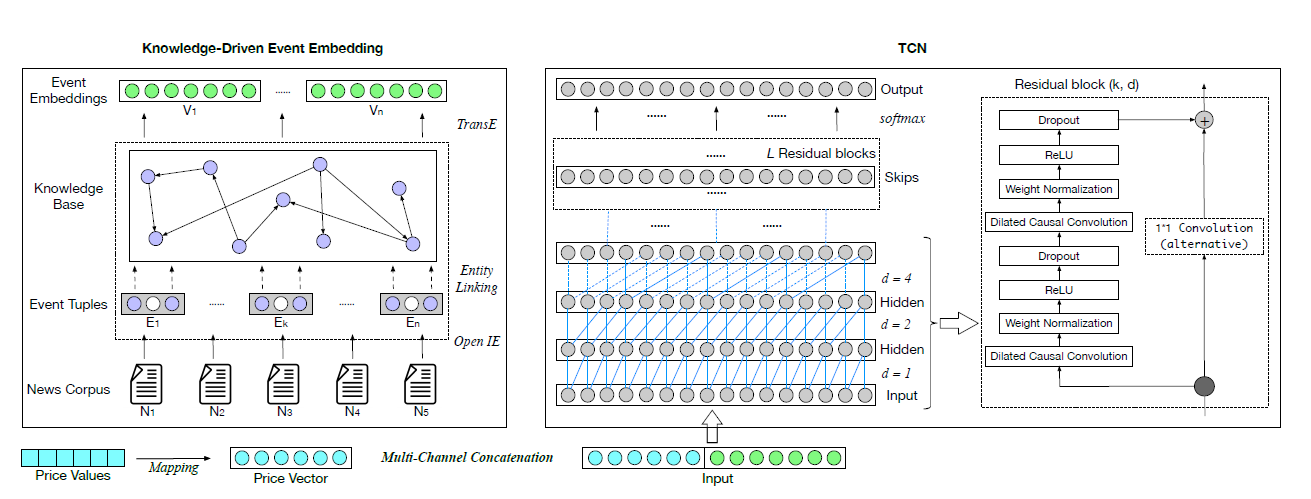
\includegraphics[width=\textwidth]{../Figures/ch_3_11_1.png}
    \caption{KDTCN model}
\end{figure}

In the KDTCN architecture, the original model inputs are price values $\mathcal{X}$ , news corpus $\mathcal{N}$ , and knowledge graph $\mathcal{G}$. The price values are normalized and mapped into the price vector, denoted by
$$\mathcal{P}=\{p_0,p_1,\ldots,p_{T-1}\}$$
where each vector $p_t$ represents a real-time price vector on a stock trading day $t$ , and $T$  is the time span. Pieces of news are represented as event sets $\mathcal{E}$ , and event tuple is defined as $ e = (s,p, o)$, where $p$  is the action or predicate, $s$ is the actor or subject and $o$  is the object on which the action is performed. Then, each item in event tuples is linked to KG. Note that event items in this paper refer to the $s$, $p$ and $o$ ,  and  in the event tuple $(s, p, o)$ , and they also correspond to entities and relations in KG. They obtain event embeddings $\mathcal{V}$  by training both event tuples and KG triples. 
They propose $linking(e)$ and $linking(r)$ to define the entity and relation in an event tuple linked to KG, as well as $context\ (e)$ to define the immediate neighbors of linked entities in KG, denoted by
$$linking\left(e\right)={\{e}_i|e_i=s\vee o,\left(s,p,o\right)\in\mathcal{E}_t\land e_i\in\mathcal{G}\ \}$$ $$linking\left(r\right)=\{r_i|r_i=p\land\left(s,p,o\right)\in\mathcal{E}_t\land r_i\in\mathcal{G}\}$$
$$context\ (e)\ =\ \{e_i\ |\ (e_i\ ,\ r\ ,\ e)\ \in\ \mathcal{G}\ \vee\ (e,\ r\ ,\ e_i\ )\ \in\ \mathcal{G},\ e\ \in\ linking(e)\}$$

Then they parameterize event representations in different channels, denoted by $\mathcal{V}_l$ in the channel of KG linking,  $\mathcal{V}_c$ in the channel of KG context, and $\mathcal{V}_w$  in the channel of words.
$$\mathcal{V}_l=\left[\mathcal{V}_{e_l^s\ },\mathcal{V}_{r_l^p\ },\mathcal{V}_{e_l^o\ }\right]$$
$$\mathcal{V}_c=\left[\mathcal{V}_{e_c^s\ },\mathcal{V}_{r_c^p\ },\mathcal{V}_{e_c^o\ }\right]$$
$$\mathcal{V}_w=\left[\mathcal{V}_{e_w^s\ },\mathcal{V}_{r_w^p\ },\mathcal{V}_{e_w^o\ }\right]$$
where $e_l^s,e_l^o\in linking\left(e\right)$, and ${\ r}_l^p\in linking\left(r\right)$; $e_c^s,e_c^o\in context\left(e\right)$ , and $r_c^p\ \in\mathcal{G}$;  $\mathcal{V}_{e_w^s\ },\mathcal{V}_{r_w^p\ }$ and $\mathcal{V}_{e_w^o\ }$  are the word vectors of $s$, $p$ and $o$ respectively; $\mathcal{V}_\ast$ represents the embedding of $∗$. Then we concatenate $\mathcal{V}_l$, $\mathcal{V}_c $ ,  and $\mathcal{V}_w$   in multiple channels to get the final event embedding, denoted by
$$\mathcal{V}=F_e\left(\mathcal{E},\mathcal{G}\right)=\left[\mathcal{V}_l{\ \mathcal{V}}_c{\ \mathcal{V}}_w\right]$$
Finally, event embeddings, combined with price vectors are input into a TCN-based model for stock trend prediction and explanation particularly with abrupt changes.

\section{Attention Mechanism}

Several papers have studied using basic and modified attention mechanisms for time series data. LSTNet (Guokun Lai (2018)) is one of the papers that proposes using an LSTM with attention mechanism for multivariate forecasting time series. Temporal Pattern Attention for Multivariate Time Series Forecasting by Shun-Yao Shih et al. focused on applying attention specifically for multivariate data. This mechanism aimed to resolve issues including noisy variables in the multivariate time series and introduce a better method than a simple average. Neo Wu et al.(2020) employed Transformer-based machine learning models to forecast time series data. This approach works by leveraging self-attention mechanisms to learn complex patterns and dynamics from time-series data. 
% Chapter 3

\chapter{Experiment 1} % Main chapter title

\label{Chapter3} % For referencing the chapter elsewhere, use \ref{Chapter1} 

%----------------------------------------------------------------------------------------

In this report, we denote our experiment of reproducing existed works, including Shaojie Bai(2018), Alberto Gasparin(2019), as "Experiment 1". And the reasons to do such a reimplement are list following.

As we addressed in \ref{Chapter1}, there are many kinds of data have the feature successive in time in common, and scholars from different research area contributed multiple views, methods, and tools to do modeling; so it is quite massive for us to have a concise plan for further work if we go through papers one by one. Instead, we will use serval mainstream models(that are introducted in \ref{Chapter2}) and apply them to different kinds of data sets. And we also want to find an ideal data set for further experiments and implement our own research framework through such a simple reproducing and comparison. 

\section{Programming Environment}
We will use Python3 with Pandas, Numpy, and TensorFlow packages for all experiments in this project. And we use CityU Burgundy HPC as part of our hardware supports.

\section{Data Processing}

\subsection{Sequential MNIST}
\subsection{JSB Chorales, Music}
\subsection{PennTreebank, LM}
\subsection{Dow Jones Industrial Average, Finance}

\section{Code Design}


\section{Numeric results}

% Chapter 4

\chapter{Time series anomaly detection in grid load issue} % Main chapter title

\label{Chapter4} % For referencing the chapter elsewhere, use \ref{Chapter1} 
\setlength{\parindent}{0pt}
%----------------------------------------------------------------------------------------

\section{Data Description}
We will try to model and refine our predictions and detections on electronic grid load issues with the base of understanding existing models and characters of kinds of data set. There are two kinds of reasons to choose such a special problem to solve. One is that compared to other kinds of sequential data; grid load data is relatively stable and cyclic. This feature makes it more factorable to label or locate "anomaly period" so that our model could have more application beyond one certain dataset. On the other hand, all the datasets in Chapter3 we have tested are offered by university labs and commonly used in machine learning tasks. They were elaborative preprocessed already and might make significance in new model checking than application. 

For grid load data, anomaly detection is useful but might be ignored by many analysts. Not only to deal with grid supply smarter, energy-saving, and could prevent fire caused by over-electricity load, but also, could be used into crime capture or financial evaluations(like loan limitations for factories), because nearly all the activities need electronic equipment and once we detect anomaly load in some subsection of the grid, i.e., distinct or state levels, might reflect some vital changes in producing or daily lives. 

We used GEFCom2014 (Electric load forecasting) as our mainly dataset to train our models, a probabilistic energy forecasting competition with four tracks on load, price, wind and solar forecasting, which attracted 581 participants from 61 countries. And we draw a basic trends plot for it, as Figure \ref{fig:gefc2014} shows.

% \begin{figure}[H]
%     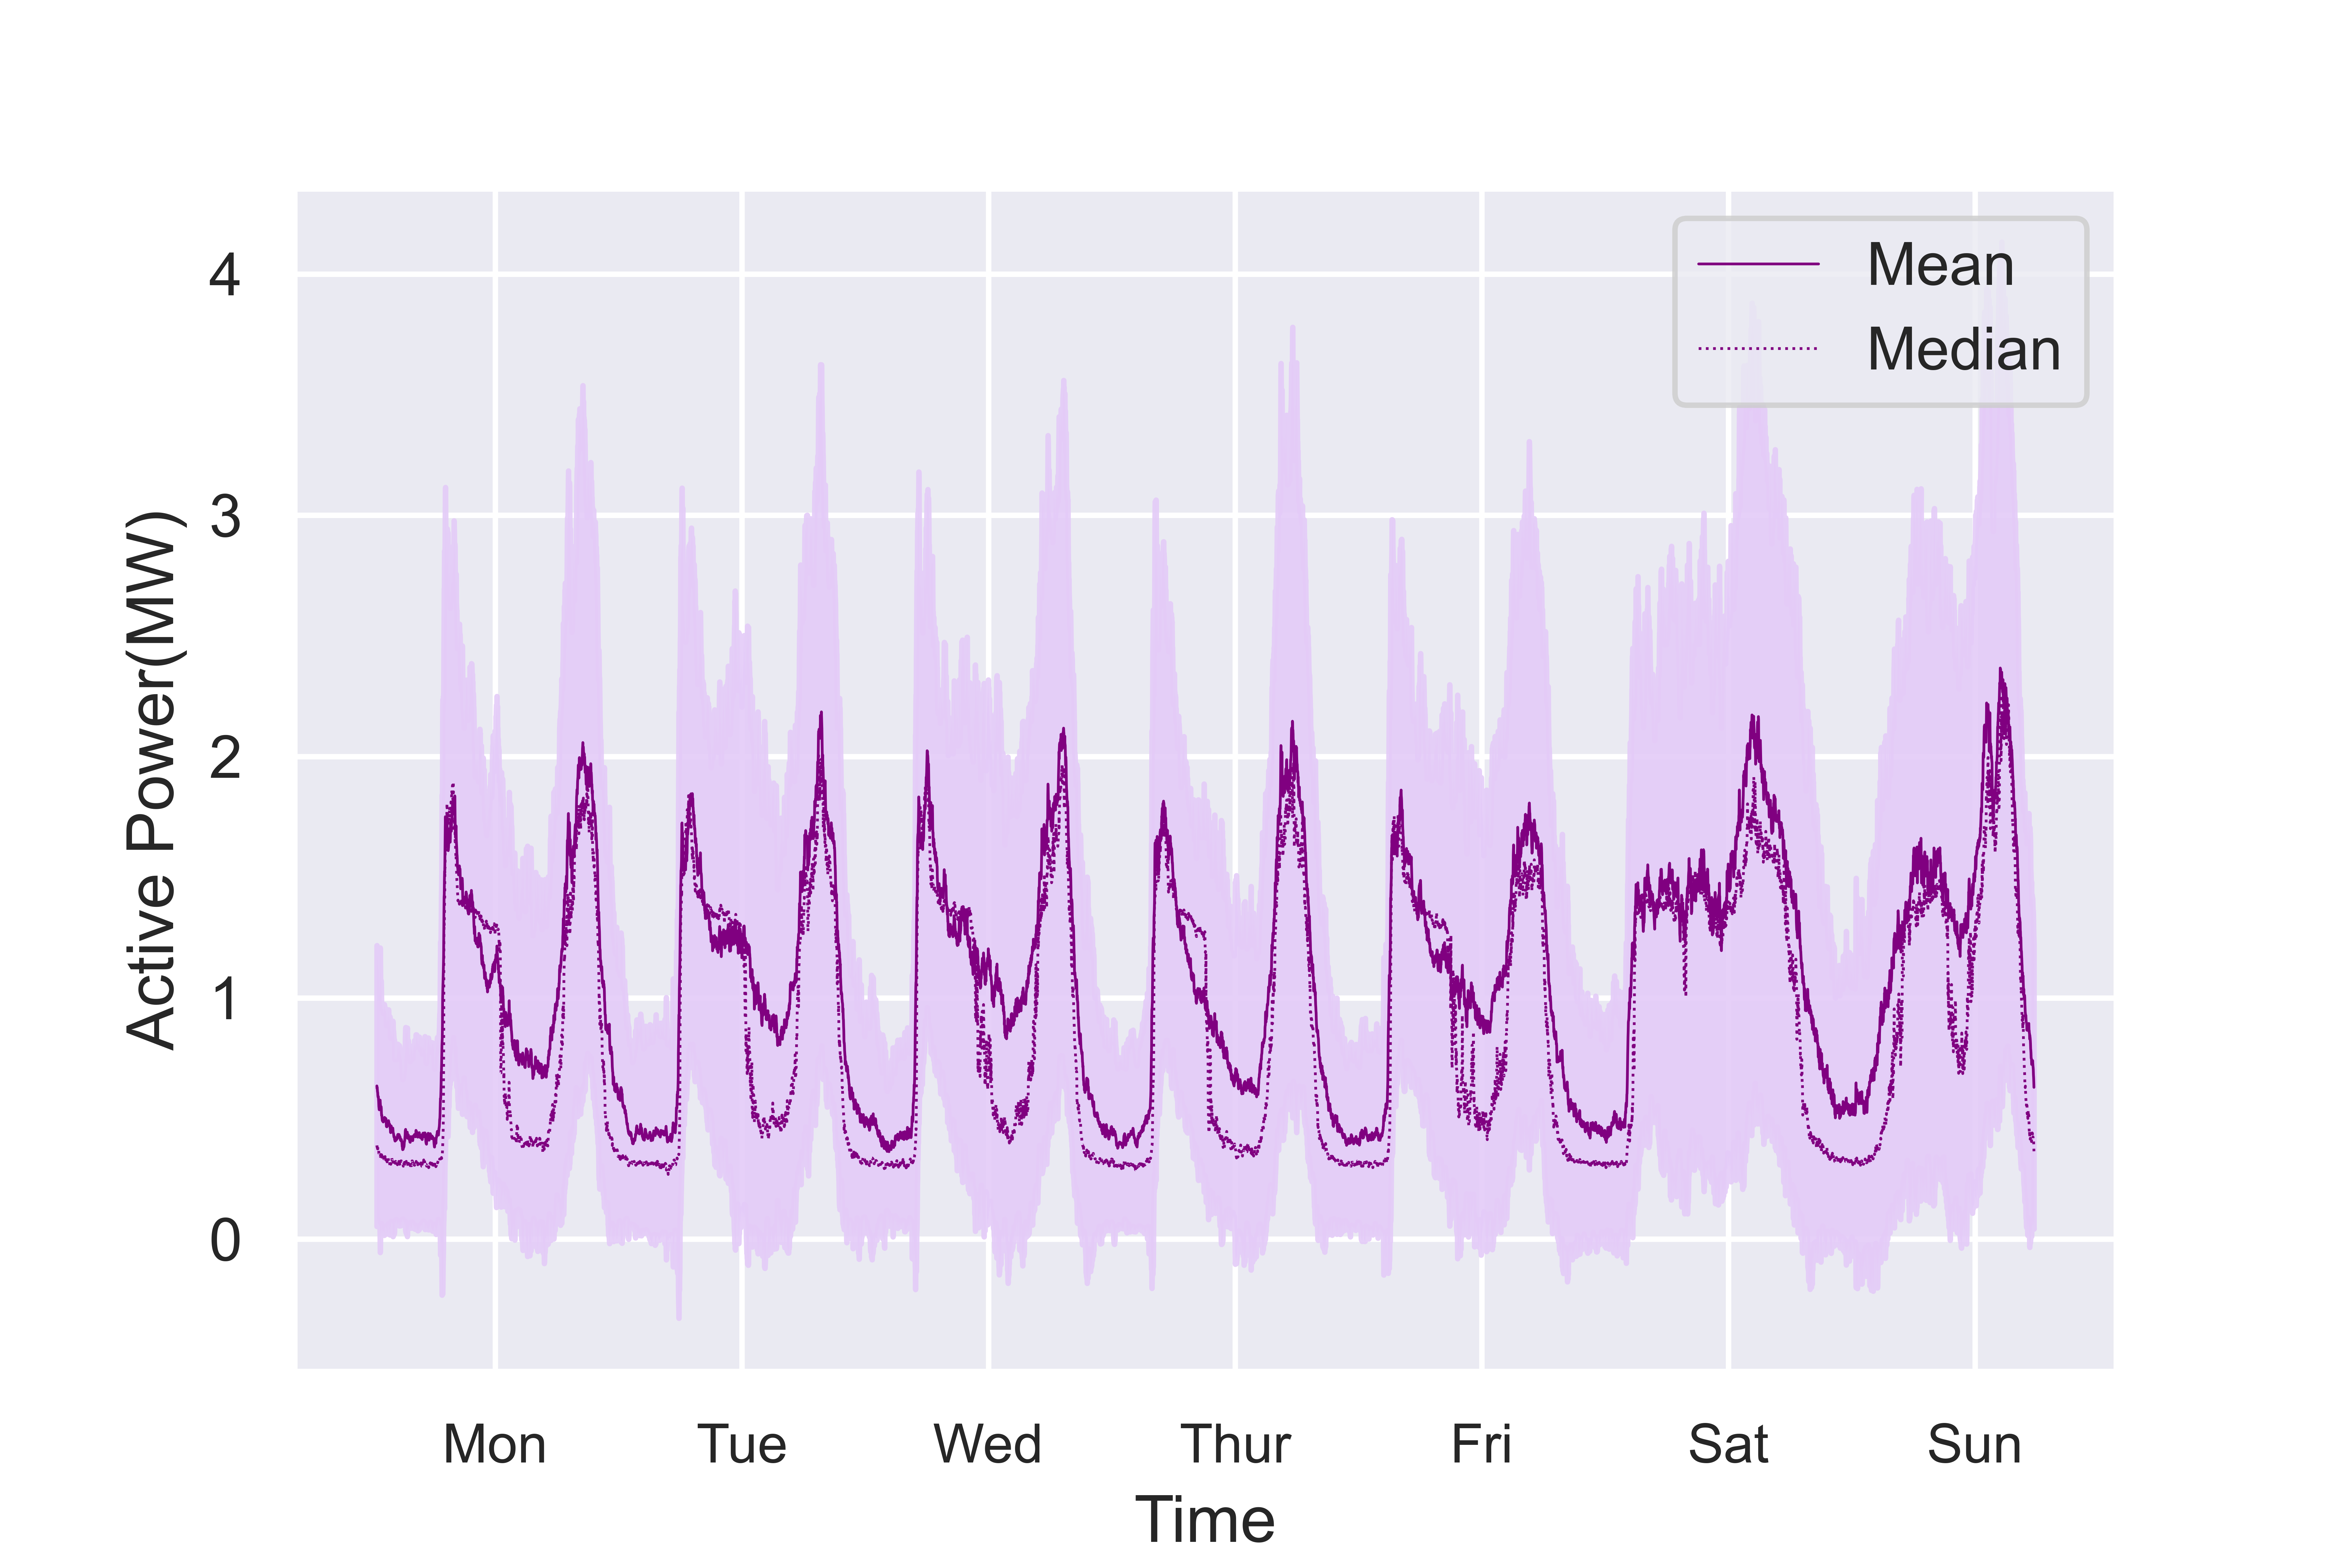
\includegraphics[width=\textwidth]{../Figures/uci.PNG}
% \end{figure}

\begin{figure}[H]
    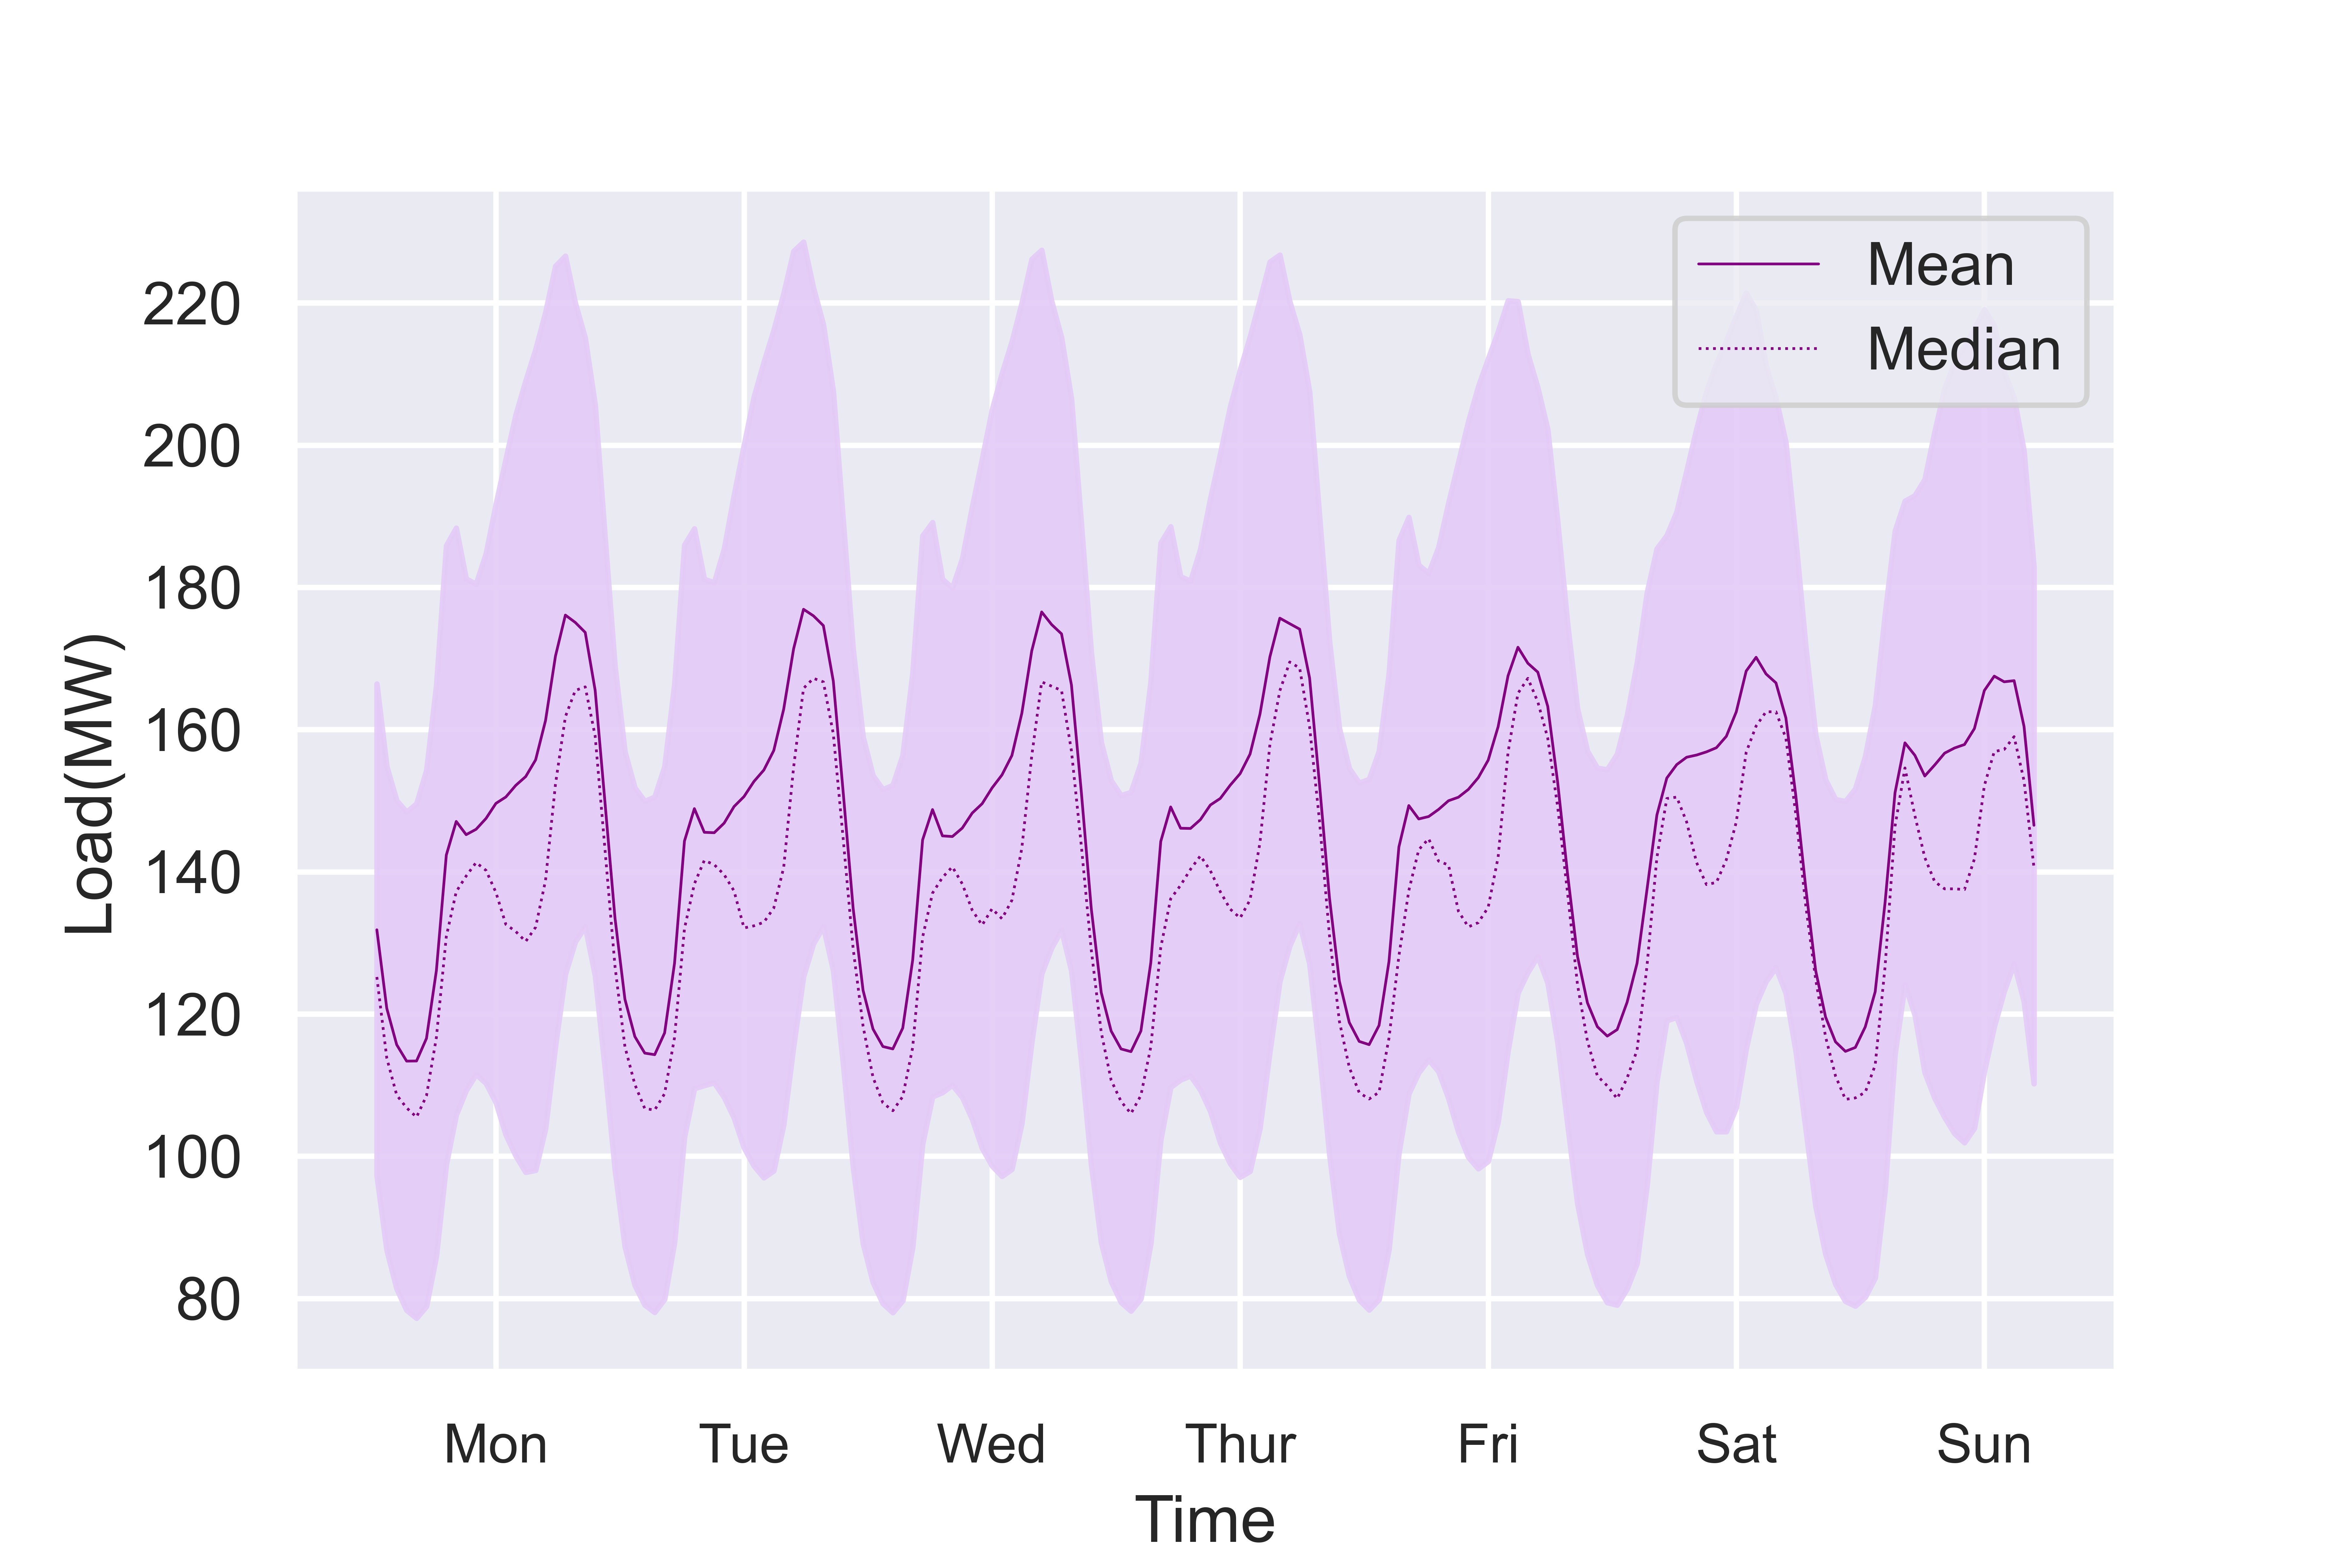
\includegraphics[width=\textwidth]{../Figures/gef2014.PNG}
    \caption{GEFCom2014 Electric Load}
    \label{fig:gefc2014}
\end{figure}

\section{Models and Evaluation}
In this experiment, TCN together with FNN, RNN, GRU, seq2seq models were adopted. And we use $MSE$,$RMSE$, $MAE$ and $R^2$ to evaluate models' performance. Besides, we also try to evaluate detection accuracy by using \textit{long-short prediction difference(LSPD)}. The definitions of these metrics are noted below.

$$RMSE = \sqrt[2]{\frac{1}{N}\sum_{i=0}^{N-1}\frac{1}{n_o}\sum_{t=0}^{n_o-1}(\hat{y_i}[t]-y_i[t])^2} $$
$$MAE = \frac{1}{N}\sum_{i=0}^{N-1}\frac{1}{n_o}\sum_{t=0}^{n_o-1}|\hat{y_i}[t]-y_i[t]|$$
$$R^2 = \frac{1}{N}\sum_{i=0}^{N-1}(1- \frac{RSS}{TSS})$$
$$RSS=\frac{1}{n_o}\sum_{t}^{n_o}(\hat{y_i}[t]-y_i[t])^2 \quad TSS= \frac{1}{n_o}\sum_{t}^{n_o}(y_i[t] - \overline{y}_i)^2 $$
$$MSE = \frac{1}{N}\sum_{i=0}^{N-1}\frac{1}{n_o}\sum_{t=0}^{n_o-1}(\hat{y_i}[t]-y_i[t])^2$$


\section{Programming Environment and Experiment Settings}
We adopted Keras framework to help us build such a experiment, related hardware and software dependencies as following table \ref{tab:dependencies}. 

\begin{table}[H]
\centering
\caption{Hardware and software dependencies}
\begin{tabular}{l l}
\toprule
\textbf{Item} & \textbf{Dependencies}  \\
\midrule
Cloud Computation Support & Supported by CityU Burgundy HPC\\
Python & Version 3.6.x  \\
TensorFlow& Version 2.1 \\
Keras& 2.3.1 \\
sacred& 0.7.5 \\
\bottomrule
\end{tabular}
\label{tab:dependencies}
\end{table}

\section{Numeric Results and Discussion}

\subsection{Models' performance comparison}
\begin{table}[H]
\centering
\caption{Models' Performance Comparison}
\begin{tabular}{l r r r r}
\toprule
\textbf{Model} & \textbf{MSE} & \textbf{MAE} & \textbf{$R^2$}& \textbf{RMSE}\\
\midrule
TCN & 772.69& 18.57& 0.86& 27.80\\
GRU\-Rec & 746.99& 19.64& 0.79& 27.33 \\
GRU\-MIMO& 423.54& 15.50& 0.82& 20.58 \\
Vanilla RNN& 2275.85& 30.47& 0.73& 47.71 \\
LSTM\-Rec & 697.94& 24.65& 0.76& 26.42 \\
LSTM\-MIMO & 378.31& 16.18& 0.87& 19.45 \\
FNN & 330.90& 10.53& \color{red}0.88& 18.19 \\
\bottomrule
\end{tabular}
\label{tab:models}
\end{table}

From table \ref{tab:models} we can find that FNN shows the best fit result amongst all the models we have adopted, with the $R^2 = 0.88$. Since TCN did not reach a good detection performance as other models did, so we did more sub-experiments on TCN, mainly on hyper-parameters modification and different datasets (not yet).

\begin{figure}[htbp]
\centering
\subfloat[fnn1]{
    \begin{minipage}[t]{0.5\textwidth}
    \centering
    \includegraphics[width=6.5cm]{reports/Figures/fnn-1.png}
    \end{minipage}
}
\subfloat[fnn2]{
    \begin{minipage}[t]{0.5\textwidth}
    \centering
    \includegraphics[width=6.5cm]{reports/Figures/fnn-2.png}
    \end{minipage}
}

\subfloat[fnn3]{
    \begin{minipage}[t]{0.5\textwidth}
    \centering
    \includegraphics[width=6.5cm]{reports/Figures/fnn-3.png}
    \end{minipage}
    }
\subfloat[fnn4]{    
    \begin{minipage}[t]{0.5\textwidth}
    \centering
    \includegraphics[width=6.5cm]{reports/Figures/fnn-4.png}
    \end{minipage}
}
\caption{Plots of FNN results} 
\label{FNN}%                         
\end{figure}

\begin{figure}[htbp]
\centering
\subfloat[tcn1]{
    \begin{minipage}[t]{0.48\textwidth}
    \centering
    \includegraphics[width=6.5cm]{reports/Figures/tcn-1.png}
    \end{minipage}
}
\subfloat[tcn2]{
    \begin{minipage}[t]{0.48\textwidth}
    \centering
    \includegraphics[width=6.5cm]{reports/Figures/tcn-2.png}
    \end{minipage}
}

\subfloat[tcn3]{
    \begin{minipage}[t]{0.48\textwidth}
    \centering
    \includegraphics[width=6.5cm]{reports/Figures/tcn-3.png}
    \end{minipage}
    }
\subfloat[tcn4]{    
    \begin{minipage}[t]{0.48\textwidth}
    \centering
    \includegraphics[width=6.5cm]{reports/Figures/tcn-4.png}
    \end{minipage}
}
\caption{Plots of TCN results} 
\label{TCN}%                         
\end{figure}

\begin{figure}[htbp]
\centering
\subfloat[gru-mimo1]{
    \begin{minipage}[t]{0.48\textwidth}
    \centering
    \includegraphics[width=6.5cm]{reports/Figures/gru-mimo-1.png}
    \end{minipage}
}
\subfloat[gru-mimo2]{
    \begin{minipage}[t]{0.48\textwidth}
    \centering
    \includegraphics[width=6.5cm]{reports/Figures/gru-mimo-2.png}
    \end{minipage}
}

\subfloat[gru-mimo3]{
    \begin{minipage}[t]{0.48\textwidth}
    \centering
    \includegraphics[width=6.5cm]{reports/Figures/gru-mimo-3.png}
    \end{minipage}
    }

\caption{Plots of GRU-MIMO results} 
\label{GRU-MIMO}%                         
\end{figure}

% \begin{figure}
%     \centering
%     \begin{subfigure}[b]{0.55\textwidth}
%         \centering
%         \includegraphics[width=\textwidth]{../Figures/fnn-1.png}
%         \caption{fnn1}
%         \label{fig:fnn1}
%     \end{subfigure}
%     \hfill
%     \begin{subfigure}[b]{0.55\textwidth}
%         \centering
%         \includegraphics[width=\textwidth]{../Figures/fnn-2.png}
%         \caption{fnn2}
%         \label{fig:fnn2}
%     \end{subfigure}
%     \hfill
%     \begin{subfigure}[b]{0.55\textwidth}
%         \centering
%         \includegraphics[width=\textwidth]{../Figures/fnn-3.png}
%         \caption{fnn3}
%         \label{fig:fnn3}
%     \end{subfigure}
%     \hfill
%     \begin{subfigure}[b]{0.55\textwidth}
%         \centering
%         \includegraphics[width=\textwidth]{../Figures/fnn-4.png}
%         \caption{fnn4}
%         \label{fig:fnn4}
%     \end{subfigure}
%       \caption{FNN results in plot}
%       \label{fig:fnn}
% \end{figure}


% \begin{figure}
%     \centering
%     \begin{subfigure}[b]{0.55\textwidth}
%         \centering
%         \includegraphics[width=\textwidth]{../Figures/tcn-1.png}
%         \caption{tcn1}
%         \label{fig:tcn1}
%     \end{subfigure}
%     \hfill
%     \begin{subfigure}[b]{0.55\textwidth}
%         \centering
%         \includegraphics[width=\textwidth]{../Figures/tcn-2.png}
%         \caption{tcn2}
%         \label{fig:tcn2}
%     \end{subfigure}
%     \hfill
%     \begin{subfigure}[b]{0.55\textwidth}
%         \centering
%         \includegraphics[width=\textwidth]{../Figures/tcn-3.png}
%         \caption{tcn3}
%         \label{fig:tcn3}
%     \end{subfigure}
%     \hfill
%     \begin{subfigure}[b]{0.55\textwidth}
%         \centering
%         \includegraphics[width=\textwidth]{../Figures/tcn-4.png}
%         \caption{tcn4}
%         \label{fig:tcn4}
%     \end{subfigure}
%       \caption{TCN results in plot}
%       \label{fig:tcn}
% \end{figure}

% \begin{figure}
%     \centering
%     \begin{subfigure}[b]{0.55\textwidth}
%         \centering
%         \includegraphics[width=\textwidth]{../Figures/gru-mimo-1.png}
%         \caption{gru-mimo1}
%         \label{fig:gru-mimo1}
%     \end{subfigure}
%     % \hfill
%     \begin{subfigure}[b]{0.55\textwidth}
%         \centering
%         \includegraphics[width=\textwidth]{../Figures/gru-mimo-2.png}
%         \caption{gru-mimo2}
%         \label{fig:gru-mimo2}
%     \end{subfigure}
%     % \hfill
%     \begin{subfigure}[b]{0.55\textwidth}
%         \centering
%         \includegraphics[width=\textwidth]{../Figures/gru-mimo-3.png}
%         \caption{gru-mimo3}
%         \label{fig:gru-mimo3}
%     \end{subfigure}
%       \caption{GRU-MIMO results in plot}
%       \label{fig:gru-mimo}
% \end{figure}


\subsection{TCN Improvement}
\begin{table}[H]
\centering
\caption{Hyper Parameters Comparison}
\begin{tabular}{l r r r r r r r r r r  r r r}
\toprule
\textbf{Test} & \textbf{Epochs} & \textbf{Input} & \textbf{Output}& \textbf{Lrate} & \textbf{L2-reg} & \textbf{OChannel} & \textbf{MSE} & \textbf{MAE} & \textbf{$R^2$}& \textbf{RMSE} \\
\midrule
Raw & 1& 96& 24& 0.001& 0.005& 32& 772.69& 18.57& 0.54& 27.80\\
T1 & \color{blue}100& 96& 24& 0.001& 0.005& 32& 280.32& 10.38& 0.84& 16.74 \\
T2 & \color{blue}30& 24& 24& 0.001& 0.005& 32& 315.89& 10.83& 0.82& 17.77 \\
T3 & 30& \color{blue}48& 24& 0.001& 0.005& 32& 300.18& 10.58& 0.83& 17.33 \\
T4 & 30& \color{blue}96& 24& 0.001& 0.005& 32& 280.32& 10.38& 0.84& 16.74 \\
T5 & 30& \color{blue}168& 24& 0.001& 0.005& 32& 300.18& 10.58& 0.83& 17.33 \\
T6 & 30& \color{blue}336& 24& 0.001& 0.005& 32& 259.50& 9.91& 0.84& 16.11 \\ %14
T7 & 30& 336& \color{blue}48& 0.001& 0.005& 32& 370.97& 11.80& 0.76& 19.26 \\
T8 & 30& 168& 24& \color{blue}0.01& 0.005& 32& 265.36& 10.03& 0.84& 16.29 \\
T9 & 30& 168& 24& 0.001& \color{blue}0.001& 32& 256.22& 9.81& 0.86& 16.01 \\
T10 & 30& 168& 24& 0.001& \color{blue}0.01& 32& 266.83& 9.81& 0.84& 16.34 \\
T11 & 30& 168& 24& 0.001& 0.01& \color{blue}16& 254.09& 9.61& \color{red}0.864& 15.94 \\
\bottomrule
\end{tabular}
\label{tab:hyper}
\end{table}

As table \ref{tab:hyper} showed, we try to change input length and output length , which are how many hours will be used as a sliding window's input and output, to make the model more sensible, and according to test metrics, we found that TCN will give the best performance when we try to use 7 days (168 hours)' electricity load to predict one day(24 hours)'s electricity load, we got $R^2 \geq 0.85$.

As for Epochs, which means the number of passes of the entire training dataset the deep learning algorithm has completed, significantly influenced TCN's training, and 30 epochs will give the most economical training results. We guess this is because TCN needs more passes to fit a good state, for it lacks some mechanism like LSTM's recurrent units.

Learning rate, L2-regulation, and the number of out channels were also influenced, but they mainly contributed to improving computation speed.

% \newpage
\section{Further Discussion with Dataset Sensitivity of TCN and LSTM }
From the previous experiment result, the TCN model present a good performance with whole Gefcom2014 dataset, but it’s not the most outstanding one. Then here are some assumptions coming up: \\
1. Is the TCN would perform better in a high variance dataset than a low variance dataset, in other word, have a better performance on anomaly detection; \\
2. How much the size of dataset would influence the TCN fitted result. 
\subsection{Experiment on different variance data}
In order to find specific effects on different variance of data with TCN, we create four datasets derived from original Gefcom2014 data as object data, each data has different variance. The plots of the four datasets are below:

\begin{figure}[htbp]
\centering
\subfloat[data1]{
    \begin{minipage}[t]{0.48\textwidth}
    \centering
    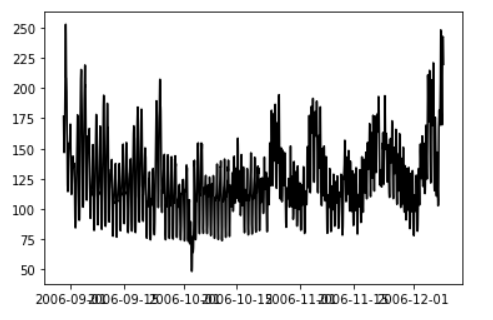
\includegraphics[width=6.5cm]{reports/Figures/data1.PNG}
    \end{minipage}
}
\subfloat[data2]{
    \begin{minipage}[t]{0.48\textwidth}
    \centering
    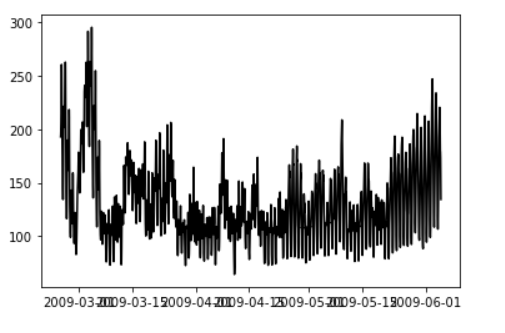
\includegraphics[width=6.5cm]{reports/Figures/data2.PNG}
    \end{minipage}
}

\subfloat[data3]{
    \begin{minipage}[t]{0.48\textwidth}
    \centering
    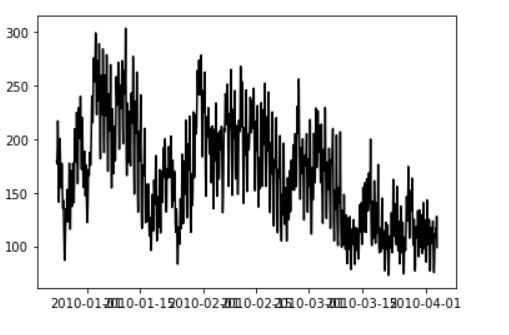
\includegraphics[width=6.5cm]{reports/Figures/data3.PNG}
    \end{minipage}
    }
\subfloat[data4]{    
    \begin{minipage}[t]{0.48\textwidth}
    \centering
    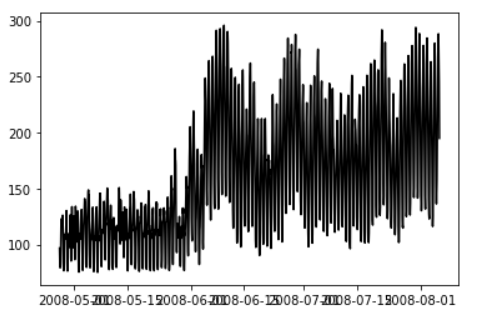
\includegraphics[width=6.5cm]{reports/Figures/data4.PNG}
    \end{minipage}
}
\caption{Plots of datasets} 
\label{Plots of datasets}%                         
\end{figure}

By applying TCN on datas, we get experiment results as below, and we use $R^2$ as measurement.
\begin{table}[H]
\centering
\caption{TCN Performance Comparison 1}
\begin{tabular}{l r r r r}
\toprule
\textbf{data}  & \textbf{data variance}& \textbf{$R^2$} & \textbf{epoch}& \textbf{stable epoch}\\
\midrule
data1 & 928.38 & 0.7201& 150& 110\\
data2 & 1380.28 & 0.7586& 150& 110 \\
data3 & 2263.21 & 0.9246& 150& 10 \\
data4 & 3200.74 & 0.7805& 150& 70 \\
\bottomrule
\end{tabular}
\label{tab:TCN}
\end{table}

In the table the 'stable epoch' means the amount of epochs the model needed to iterate and attain a stable $R^2$ value. From the results we find that with high variance data, TCN do perform better on $R^2$, which represent that TCN model is more sensitive to detect anomaly in time series data. However, for data3, the variance of it is not greater than data4, while the corresponding $R^2$ is higher. By comparing the data shape above, we can find that data4 is more likely a data merged by two stable datasets with a sharp connection between them, while data3 is a real fluctuated data. \\
And as LSTM also performs well with original data in previous experiment, we try to apply it on the four datasets as comparison. In order to make comparison the more convincing, most of the hyper-parameters in two models are stay the same. The results are shown below:
\begin{table}[H]
\centering
\caption{LSTM Performance Comparison 1}
\begin{tabular}{l r r r r}
\toprule
\textbf{data}  & \textbf{data variance}& \textbf{$R^2$} & \textbf{epoch}& \textbf{stable epoch}\\
\midrule
data1 & 928.38 & 0.7161 & 50& 30\\
data2 & 1380.28 & 0.7637 & 50& 30 \\
data3 & 2263.21 & 0.8385 & 50& 30 \\
data4 & 3200.74 & 0.7761 & 50& 30 \\
\bottomrule
\end{tabular}
\label{tab:LSTM}
\end{table}
The results show that LSTM also performs better in high variance data, and the $R^2$ in data3 is also greater than data4. but the $R^2$ improvement from low variance data to high variance data is not as much as TCN. The difference may because that in TCN, convolutional layer used to extract features, so that in fluctuated dataset, it would easier to extract useful features and improve the model performance, while in flatter dataset, it's advantage can not be applied and can hardly outperform other NN algorithms.
\subsection{Experiment on different size data}
In order to find specific effects on different size of data with TCN, we create four datasets derived from original Gefcom2014 data as training data, each data has different data size. The plots of the four datasets are below:
\begin{figure}[H]
\centering
\subfloat[data5]{
    \begin{minipage}[t]{0.48\textwidth}
    \centering
    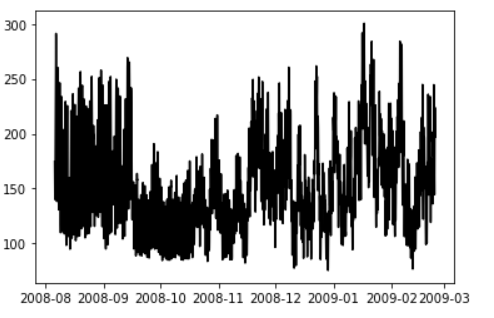
\includegraphics[width=6.5cm]{reports/Figures/data5.PNG}
    \end{minipage}
}
\subfloat[data6]{
    \begin{minipage}[t]{0.48\textwidth}
    \centering
    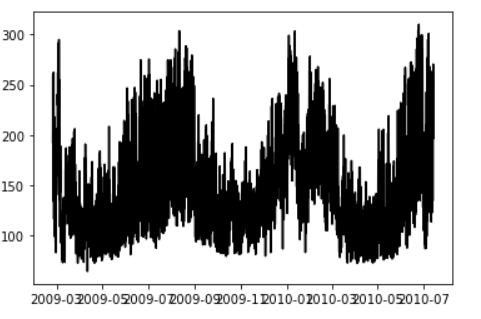
\includegraphics[width=6.5cm]{reports/Figures/data6.PNG}
    \end{minipage}
}

\subfloat[data7]{
    \begin{minipage}[t]{0.48\textwidth}
    \centering
    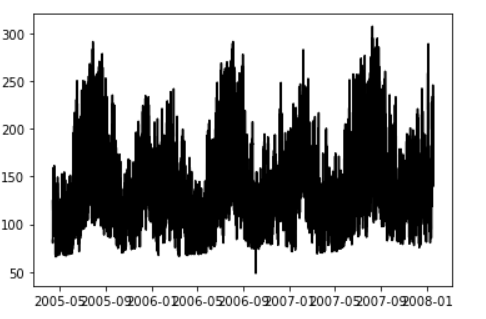
\includegraphics[width=6.5cm]{reports/Figures/data7.PNG}
    \end{minipage}
    }
\subfloat[data8]{    
    \begin{minipage}[t]{0.48\textwidth}
    \centering
    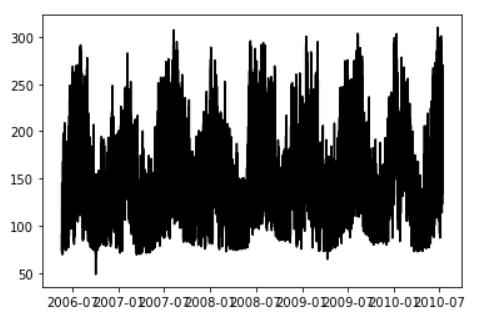
\includegraphics[width=6.5cm]{reports/Figures/data8.PNG}
    \end{minipage}
}
\caption{Plots of datasets 2} 
\label{Plots of datasets 2}%                         
\end{figure}
By applying TCN on datasets, we get experiment results as below:
\begin{table}[H]
\centering
\caption{TCN Performance Comparison 2}
\begin{tabular}{l r r r r}
\toprule
\textbf{data}  & \textbf{data size}& \textbf{$R^2$} & \textbf{epoch}& \textbf{stable epoch}\\
\midrule
data5 & 4848 & 0.7525 & 150& 70\\
data6 & 12120 & 0.8587 & 150& 30 \\
data7 & 24240 & 0.8591 & 150& 10 \\
data8 & 36360 & 0.8607 & 150& 10 \\
original data & 60600 & 0.8641& 150& 10 \\
\bottomrule
\end{tabular}
\label{tab:TCN2}
\end{table}
For long-term dataset, TCN would easily get a good fitted result with only 10 epochs training, while for short-term dataset, TCN perform worse and need more than 70 epochs training to provide a relatively good result.\\
And we also apply the same datas into LSTM model, here is table of LSTM training results:
\begin{table}[H]
\centering
\caption{LSTM Performance Comparison 2}
\begin{tabular}{l r r r r}
\toprule
\textbf{data}  & \textbf{data size}& \textbf{$R^2$} & \textbf{epoch}& \textbf{stable epoch}\\
\midrule
data5 & 4848 & 0.8149 & 50& 30\\
data6 & 12120 & 0.8441 & 50& 20 \\
data7 & 24240 & 0.8656 & 50& 10 \\
data8 & 36360 & 0.8674 & 50& 10 \\
original data & 60600 & 0.8763& 50& 10 \\
\bottomrule
\end{tabular}
\label{tab:LSTM2}
\end{table}
For the $R^2$ of long-term data and short-term data, LSTM also get a lower improvement compared to TCN, which means that TCN is more sensitive to the data size. However, when faced a small dataset, LSTM need fewer epochs to attain the relative optimal point than TCN, which indicates that LSTM would be more efficient in time series data training while applying on small sample. One of the reasons is that TCN model have convolutional layers with more parameters need to be iterated. When LSTM is processing, only one hidden state need to be concentrate on and every state get one single input, while for TCN, it request a long enough sequence to keep the history state, which require a bigger memory. However, since the same filter is used in each layer, convolutions can be done in parallel, so that TCN would be more efficient on huge dataset instead of small dataset. \\

\section{Discussion with kernel adjustment and improved performance}
In the previous discussion, we find TCN perform worse for short-term dataset than long-term dataset, and will take more training epochs to provide a relatively good result, which indicates that TCN is more sensitive to the data size and also time-consuming although it allows for parallel computation of outputs. In order to improve this problem, we did some adjustment to our convolutional kernel to have a bigger receptive field. The architecture of TCN employs dilated convolutions that enable an exponentially large receptive field. Using larger dilation enables an output at the top level to represent a wider range of inputs, there are two ways to increase the receptive field size of TCN: choosing lager filter sizes k and increasing the dilation factor d. After doing some adjustment to TCN's convolutional kernel, the updated result is shown below:

\begin{table}[H]
\centering
\caption{TCN's Kernel Adjustment Performance comparison}
\begin{tabular}{l r r r r}
\toprule
\textbf{Test}  & \textbf{dilation}& \textbf{kernel size} & \textbf{epochs}& \textbf{$R^2$}\\
\midrule
Raw & 2 & 2 & 30 & 0.8521\\
T1 & \color{blue}1 & 2 & 30 & 0.8498 \\
T2 & \color{blue}3 & 2 & 30 & 0.8547 \\
T3 & \color{blue}4 & 2 & 30 & 0.8513 \\
T4 & 4 & \color{blue}3 & 30 & 0.8564 \\
T5 & 4 & \color{blue}4 & 30 & 0.8567 \\
T6 & 4 & \color{blue}5 & 30 & 0.8696 \\
T7 & 4 & \color{blue}6 & 30 & 0.8746 \\
T8 & 4 & \color{blue}7 & 30 & 0.8803 \\
T9 & \color{blue}5 & 7 & 30 & 0.8694 \\
T10 & \color{blue}6 & 7 & 30 & 0.8687 \\
Best adjustment & \textbf{\color{red}4} & \textbf{\color{red}7} & \textbf{100} & \textbf{\color{red}0.9159} \\
\bottomrule
\end{tabular}
\label{tab:LSTM2}
\end{table}

The results indicate that both dilation and kernel size can increase the receptive field size of TCN, which improves performance in varying degrees. These adjustments can help TCN reduce the dependence on sequences' length, also speed up the training process. However the performance improvements by increasing receptive field is limited, in our experiments if dilation and kernel size is bigger than some certain value, $R^2$ score will decrease a little bit instead. One of reason is that if the receptive field is too small, only local features can be observed, which is not enough to get the information of the whole sequence. If the receptive field is too large, too much noise and invalid information will be introduced which leads to worse performance. After many trials, we set dilation as 4 and kernel size as 7 and increase epochs to 100, our final and best TCN $R^2$ result is 0.9159.
\begin{table}[H]
\centering
\caption{Models' Performance Updated}
\begin{tabular}{l r r r r}
\toprule
\textbf{Model} & \textbf{MSE} & \textbf{MAE} & \textbf{$R^2$}& \textbf{RMSE}\\
\midrule
TCN & 772.69& 18.57& 0.86& 27.80\\
\textbf{TCN(kernel adjustment)} & \textbf{284.35} & \textbf{10.02} & \textbf{\color{red}0.91}& \textbf{16.88}\\
GRU\-Rec & 746.99& 19.64& 0.79& 27.33 \\
GRU\-MIMO& 423.54& 15.50& 0.82& 20.58 \\
Vanilla RNN& 2275.85& 30.47& 0.73& 47.71 \\
LSTM\-Rec & 697.94& 24.65& 0.76& 26.42 \\
LSTM\-MIMO & 378.31& 16.18& 0.87& 19.45 \\
FNN & 330.90& 10.53& 0.88& 18.19 \\
\bottomrule
\end{tabular}
\label{tab:models}
\end{table}

The result shows that TCN can achieve the best performance among all models in this electronic grid load issues. TCN model has a flexible receptive field size, which can be adjusted according to different application situation and tasks. which afford better control of the model’s memory size, and are easy to adapt to different domains. The improved TCN model is less sensitive to data size, speeds up iteration and improves predicting performance. Our result also shows that TCN can be served as a convenient but powerful starting point when dealing with sequential data.  
% Chapter 5

\chapter{Conclusion and Future Work} % Main chapter title

\label{Chapter5} % For referencing the chapter elsewhere, use \ref{Chapter1} 

%----------------------------------------------------------------------------------------

\section{Conclusion}
In our project, we first illustrate different existing research on TCN model, and find the characteristics in it. Then we checked predict ability of TCN over other relatively traditional sequential models, such as Gated recurrent units (GRUs), long short-term memory (LSTM), vanilla RNN and False nearest neighbor (FNN),  by using some specific sequence datas. And in order to have a better result, we tune the hyper parameters in TCN model. After comparison, TCN showed itself as both robust and accuracy even amongst deep learning models. However, it can not demonstrated convincing performance. Next we try to discover the data sensitivity of TCN model and add LSTM model as comparison. We find that TCN performs better than LSTM in fluctuated data. And for short data size, TCN need more time to attain a good result, while for long and huge data, TCN have ability to perform better.

\section{Further work}
However, our group still found some limitations and hope to do more improvements on following aspects:
\begin{itemize}
    \item Limited dataset. In project we tried several different datasets and choose Gefcom2014 electronic data as object dataset. The Gefcom2014 data have some good features such as regular and smooth. However, it also bring limitation to model fitting and make the experiment not that convincing. And we also need more type of data to verify the characteristics we found in TCN. So it's better for us to try more different time series data and test the finding of our project. 
    \item zone different
\end{itemize} 

%----------------------------------------------------------------------------------------
%	THESIS CONTENT - APPENDICES
%----------------------------------------------------------------------------------------

\appendix % Cue to tell LaTeX that the following "chapters" are Appendices

% Include the appendices of the thesis as separate files from the Appendices folder
% Uncomment the lines as you write the Appendices

% \include{Appendices/AppendixA}
%\include{Appendices/AppendixB}
%\include{Appendices/AppendixC}

%----------------------------------------------------------------------------------------
%	BIBLIOGRAPHY
%----------------------------------------------------------------------------------------

\printbibliography[heading=bibintoc]

%----------------------------------------------------------------------------------------

\end{document}  
